
% Default to the notebook output style

    


% Inherit from the specified cell style.




    
\documentclass[11pt]{article}

    
    
    \usepackage[T1]{fontenc}
    % Nicer default font (+ math font) than Computer Modern for most use cases
    \usepackage{mathpazo}

    % Basic figure setup, for now with no caption control since it's done
    % automatically by Pandoc (which extracts ![](path) syntax from Markdown).
    \usepackage{graphicx}
    % We will generate all images so they have a width \maxwidth. This means
    % that they will get their normal width if they fit onto the page, but
    % are scaled down if they would overflow the margins.
    \makeatletter
    \def\maxwidth{\ifdim\Gin@nat@width>\linewidth\linewidth
    \else\Gin@nat@width\fi}
    \makeatother
    \let\Oldincludegraphics\includegraphics
    % Set max figure width to be 80% of text width, for now hardcoded.
    \renewcommand{\includegraphics}[1]{\Oldincludegraphics[width=.8\maxwidth]{#1}}
    % Ensure that by default, figures have no caption (until we provide a
    % proper Figure object with a Caption API and a way to capture that
    % in the conversion process - todo).
    \usepackage{caption}
    \DeclareCaptionLabelFormat{nolabel}{}
    \captionsetup{labelformat=nolabel}

    \usepackage{adjustbox} % Used to constrain images to a maximum size 
    \usepackage{xcolor} % Allow colors to be defined
    \usepackage{enumerate} % Needed for markdown enumerations to work
    \usepackage{geometry} % Used to adjust the document margins
    \usepackage{amsmath} % Equations
    \usepackage{amssymb} % Equations
    \usepackage{textcomp} % defines textquotesingle
    % Hack from http://tex.stackexchange.com/a/47451/13684:
    \AtBeginDocument{%
        \def\PYZsq{\textquotesingle}% Upright quotes in Pygmentized code
    }
    \usepackage{upquote} % Upright quotes for verbatim code
    \usepackage{eurosym} % defines \euro
    \usepackage[mathletters]{ucs} % Extended unicode (utf-8) support
    \usepackage[utf8x]{inputenc} % Allow utf-8 characters in the tex document
    \usepackage{fancyvrb} % verbatim replacement that allows latex
    \usepackage{grffile} % extends the file name processing of package graphics 
                         % to support a larger range 
    % The hyperref package gives us a pdf with properly built
    % internal navigation ('pdf bookmarks' for the table of contents,
    % internal cross-reference links, web links for URLs, etc.)
    \usepackage{hyperref}
    \usepackage{longtable} % longtable support required by pandoc >1.10
    \usepackage{booktabs}  % table support for pandoc > 1.12.2
    \usepackage[inline]{enumitem} % IRkernel/repr support (it uses the enumerate* environment)
    \usepackage[normalem]{ulem} % ulem is needed to support strikethroughs (\sout)
                                % normalem makes italics be italics, not underlines
    

    
    
    % Colors for the hyperref package
    \definecolor{urlcolor}{rgb}{0,.145,.698}
    \definecolor{linkcolor}{rgb}{.71,0.21,0.01}
    \definecolor{citecolor}{rgb}{.12,.54,.11}

    % ANSI colors
    \definecolor{ansi-black}{HTML}{3E424D}
    \definecolor{ansi-black-intense}{HTML}{282C36}
    \definecolor{ansi-red}{HTML}{E75C58}
    \definecolor{ansi-red-intense}{HTML}{B22B31}
    \definecolor{ansi-green}{HTML}{00A250}
    \definecolor{ansi-green-intense}{HTML}{007427}
    \definecolor{ansi-yellow}{HTML}{DDB62B}
    \definecolor{ansi-yellow-intense}{HTML}{B27D12}
    \definecolor{ansi-blue}{HTML}{208FFB}
    \definecolor{ansi-blue-intense}{HTML}{0065CA}
    \definecolor{ansi-magenta}{HTML}{D160C4}
    \definecolor{ansi-magenta-intense}{HTML}{A03196}
    \definecolor{ansi-cyan}{HTML}{60C6C8}
    \definecolor{ansi-cyan-intense}{HTML}{258F8F}
    \definecolor{ansi-white}{HTML}{C5C1B4}
    \definecolor{ansi-white-intense}{HTML}{A1A6B2}

    % commands and environments needed by pandoc snippets
    % extracted from the output of `pandoc -s`
    \providecommand{\tightlist}{%
      \setlength{\itemsep}{0pt}\setlength{\parskip}{0pt}}
    \DefineVerbatimEnvironment{Highlighting}{Verbatim}{commandchars=\\\{\}}
    % Add ',fontsize=\small' for more characters per line
    \newenvironment{Shaded}{}{}
    \newcommand{\KeywordTok}[1]{\textcolor[rgb]{0.00,0.44,0.13}{\textbf{{#1}}}}
    \newcommand{\DataTypeTok}[1]{\textcolor[rgb]{0.56,0.13,0.00}{{#1}}}
    \newcommand{\DecValTok}[1]{\textcolor[rgb]{0.25,0.63,0.44}{{#1}}}
    \newcommand{\BaseNTok}[1]{\textcolor[rgb]{0.25,0.63,0.44}{{#1}}}
    \newcommand{\FloatTok}[1]{\textcolor[rgb]{0.25,0.63,0.44}{{#1}}}
    \newcommand{\CharTok}[1]{\textcolor[rgb]{0.25,0.44,0.63}{{#1}}}
    \newcommand{\StringTok}[1]{\textcolor[rgb]{0.25,0.44,0.63}{{#1}}}
    \newcommand{\CommentTok}[1]{\textcolor[rgb]{0.38,0.63,0.69}{\textit{{#1}}}}
    \newcommand{\OtherTok}[1]{\textcolor[rgb]{0.00,0.44,0.13}{{#1}}}
    \newcommand{\AlertTok}[1]{\textcolor[rgb]{1.00,0.00,0.00}{\textbf{{#1}}}}
    \newcommand{\FunctionTok}[1]{\textcolor[rgb]{0.02,0.16,0.49}{{#1}}}
    \newcommand{\RegionMarkerTok}[1]{{#1}}
    \newcommand{\ErrorTok}[1]{\textcolor[rgb]{1.00,0.00,0.00}{\textbf{{#1}}}}
    \newcommand{\NormalTok}[1]{{#1}}
    
    % Additional commands for more recent versions of Pandoc
    \newcommand{\ConstantTok}[1]{\textcolor[rgb]{0.53,0.00,0.00}{{#1}}}
    \newcommand{\SpecialCharTok}[1]{\textcolor[rgb]{0.25,0.44,0.63}{{#1}}}
    \newcommand{\VerbatimStringTok}[1]{\textcolor[rgb]{0.25,0.44,0.63}{{#1}}}
    \newcommand{\SpecialStringTok}[1]{\textcolor[rgb]{0.73,0.40,0.53}{{#1}}}
    \newcommand{\ImportTok}[1]{{#1}}
    \newcommand{\DocumentationTok}[1]{\textcolor[rgb]{0.73,0.13,0.13}{\textit{{#1}}}}
    \newcommand{\AnnotationTok}[1]{\textcolor[rgb]{0.38,0.63,0.69}{\textbf{\textit{{#1}}}}}
    \newcommand{\CommentVarTok}[1]{\textcolor[rgb]{0.38,0.63,0.69}{\textbf{\textit{{#1}}}}}
    \newcommand{\VariableTok}[1]{\textcolor[rgb]{0.10,0.09,0.49}{{#1}}}
    \newcommand{\ControlFlowTok}[1]{\textcolor[rgb]{0.00,0.44,0.13}{\textbf{{#1}}}}
    \newcommand{\OperatorTok}[1]{\textcolor[rgb]{0.40,0.40,0.40}{{#1}}}
    \newcommand{\BuiltInTok}[1]{{#1}}
    \newcommand{\ExtensionTok}[1]{{#1}}
    \newcommand{\PreprocessorTok}[1]{\textcolor[rgb]{0.74,0.48,0.00}{{#1}}}
    \newcommand{\AttributeTok}[1]{\textcolor[rgb]{0.49,0.56,0.16}{{#1}}}
    \newcommand{\InformationTok}[1]{\textcolor[rgb]{0.38,0.63,0.69}{\textbf{\textit{{#1}}}}}
    \newcommand{\WarningTok}[1]{\textcolor[rgb]{0.38,0.63,0.69}{\textbf{\textit{{#1}}}}}
    
    
    % Define a nice break command that doesn't care if a line doesn't already
    % exist.
    \def\br{\hspace*{\fill} \\* }
    % Math Jax compatability definitions
    \def\gt{>}
    \def\lt{<}
    % Document parameters
    \title{P2 Hierarchical Modeling}
    
    
    

    % Pygments definitions
    
\makeatletter
\def\PY@reset{\let\PY@it=\relax \let\PY@bf=\relax%
    \let\PY@ul=\relax \let\PY@tc=\relax%
    \let\PY@bc=\relax \let\PY@ff=\relax}
\def\PY@tok#1{\csname PY@tok@#1\endcsname}
\def\PY@toks#1+{\ifx\relax#1\empty\else%
    \PY@tok{#1}\expandafter\PY@toks\fi}
\def\PY@do#1{\PY@bc{\PY@tc{\PY@ul{%
    \PY@it{\PY@bf{\PY@ff{#1}}}}}}}
\def\PY#1#2{\PY@reset\PY@toks#1+\relax+\PY@do{#2}}

\expandafter\def\csname PY@tok@w\endcsname{\def\PY@tc##1{\textcolor[rgb]{0.73,0.73,0.73}{##1}}}
\expandafter\def\csname PY@tok@c\endcsname{\let\PY@it=\textit\def\PY@tc##1{\textcolor[rgb]{0.25,0.50,0.50}{##1}}}
\expandafter\def\csname PY@tok@cp\endcsname{\def\PY@tc##1{\textcolor[rgb]{0.74,0.48,0.00}{##1}}}
\expandafter\def\csname PY@tok@k\endcsname{\let\PY@bf=\textbf\def\PY@tc##1{\textcolor[rgb]{0.00,0.50,0.00}{##1}}}
\expandafter\def\csname PY@tok@kp\endcsname{\def\PY@tc##1{\textcolor[rgb]{0.00,0.50,0.00}{##1}}}
\expandafter\def\csname PY@tok@kt\endcsname{\def\PY@tc##1{\textcolor[rgb]{0.69,0.00,0.25}{##1}}}
\expandafter\def\csname PY@tok@o\endcsname{\def\PY@tc##1{\textcolor[rgb]{0.40,0.40,0.40}{##1}}}
\expandafter\def\csname PY@tok@ow\endcsname{\let\PY@bf=\textbf\def\PY@tc##1{\textcolor[rgb]{0.67,0.13,1.00}{##1}}}
\expandafter\def\csname PY@tok@nb\endcsname{\def\PY@tc##1{\textcolor[rgb]{0.00,0.50,0.00}{##1}}}
\expandafter\def\csname PY@tok@nf\endcsname{\def\PY@tc##1{\textcolor[rgb]{0.00,0.00,1.00}{##1}}}
\expandafter\def\csname PY@tok@nc\endcsname{\let\PY@bf=\textbf\def\PY@tc##1{\textcolor[rgb]{0.00,0.00,1.00}{##1}}}
\expandafter\def\csname PY@tok@nn\endcsname{\let\PY@bf=\textbf\def\PY@tc##1{\textcolor[rgb]{0.00,0.00,1.00}{##1}}}
\expandafter\def\csname PY@tok@ne\endcsname{\let\PY@bf=\textbf\def\PY@tc##1{\textcolor[rgb]{0.82,0.25,0.23}{##1}}}
\expandafter\def\csname PY@tok@nv\endcsname{\def\PY@tc##1{\textcolor[rgb]{0.10,0.09,0.49}{##1}}}
\expandafter\def\csname PY@tok@no\endcsname{\def\PY@tc##1{\textcolor[rgb]{0.53,0.00,0.00}{##1}}}
\expandafter\def\csname PY@tok@nl\endcsname{\def\PY@tc##1{\textcolor[rgb]{0.63,0.63,0.00}{##1}}}
\expandafter\def\csname PY@tok@ni\endcsname{\let\PY@bf=\textbf\def\PY@tc##1{\textcolor[rgb]{0.60,0.60,0.60}{##1}}}
\expandafter\def\csname PY@tok@na\endcsname{\def\PY@tc##1{\textcolor[rgb]{0.49,0.56,0.16}{##1}}}
\expandafter\def\csname PY@tok@nt\endcsname{\let\PY@bf=\textbf\def\PY@tc##1{\textcolor[rgb]{0.00,0.50,0.00}{##1}}}
\expandafter\def\csname PY@tok@nd\endcsname{\def\PY@tc##1{\textcolor[rgb]{0.67,0.13,1.00}{##1}}}
\expandafter\def\csname PY@tok@s\endcsname{\def\PY@tc##1{\textcolor[rgb]{0.73,0.13,0.13}{##1}}}
\expandafter\def\csname PY@tok@sd\endcsname{\let\PY@it=\textit\def\PY@tc##1{\textcolor[rgb]{0.73,0.13,0.13}{##1}}}
\expandafter\def\csname PY@tok@si\endcsname{\let\PY@bf=\textbf\def\PY@tc##1{\textcolor[rgb]{0.73,0.40,0.53}{##1}}}
\expandafter\def\csname PY@tok@se\endcsname{\let\PY@bf=\textbf\def\PY@tc##1{\textcolor[rgb]{0.73,0.40,0.13}{##1}}}
\expandafter\def\csname PY@tok@sr\endcsname{\def\PY@tc##1{\textcolor[rgb]{0.73,0.40,0.53}{##1}}}
\expandafter\def\csname PY@tok@ss\endcsname{\def\PY@tc##1{\textcolor[rgb]{0.10,0.09,0.49}{##1}}}
\expandafter\def\csname PY@tok@sx\endcsname{\def\PY@tc##1{\textcolor[rgb]{0.00,0.50,0.00}{##1}}}
\expandafter\def\csname PY@tok@m\endcsname{\def\PY@tc##1{\textcolor[rgb]{0.40,0.40,0.40}{##1}}}
\expandafter\def\csname PY@tok@gh\endcsname{\let\PY@bf=\textbf\def\PY@tc##1{\textcolor[rgb]{0.00,0.00,0.50}{##1}}}
\expandafter\def\csname PY@tok@gu\endcsname{\let\PY@bf=\textbf\def\PY@tc##1{\textcolor[rgb]{0.50,0.00,0.50}{##1}}}
\expandafter\def\csname PY@tok@gd\endcsname{\def\PY@tc##1{\textcolor[rgb]{0.63,0.00,0.00}{##1}}}
\expandafter\def\csname PY@tok@gi\endcsname{\def\PY@tc##1{\textcolor[rgb]{0.00,0.63,0.00}{##1}}}
\expandafter\def\csname PY@tok@gr\endcsname{\def\PY@tc##1{\textcolor[rgb]{1.00,0.00,0.00}{##1}}}
\expandafter\def\csname PY@tok@ge\endcsname{\let\PY@it=\textit}
\expandafter\def\csname PY@tok@gs\endcsname{\let\PY@bf=\textbf}
\expandafter\def\csname PY@tok@gp\endcsname{\let\PY@bf=\textbf\def\PY@tc##1{\textcolor[rgb]{0.00,0.00,0.50}{##1}}}
\expandafter\def\csname PY@tok@go\endcsname{\def\PY@tc##1{\textcolor[rgb]{0.53,0.53,0.53}{##1}}}
\expandafter\def\csname PY@tok@gt\endcsname{\def\PY@tc##1{\textcolor[rgb]{0.00,0.27,0.87}{##1}}}
\expandafter\def\csname PY@tok@err\endcsname{\def\PY@bc##1{\setlength{\fboxsep}{0pt}\fcolorbox[rgb]{1.00,0.00,0.00}{1,1,1}{\strut ##1}}}
\expandafter\def\csname PY@tok@kc\endcsname{\let\PY@bf=\textbf\def\PY@tc##1{\textcolor[rgb]{0.00,0.50,0.00}{##1}}}
\expandafter\def\csname PY@tok@kd\endcsname{\let\PY@bf=\textbf\def\PY@tc##1{\textcolor[rgb]{0.00,0.50,0.00}{##1}}}
\expandafter\def\csname PY@tok@kn\endcsname{\let\PY@bf=\textbf\def\PY@tc##1{\textcolor[rgb]{0.00,0.50,0.00}{##1}}}
\expandafter\def\csname PY@tok@kr\endcsname{\let\PY@bf=\textbf\def\PY@tc##1{\textcolor[rgb]{0.00,0.50,0.00}{##1}}}
\expandafter\def\csname PY@tok@bp\endcsname{\def\PY@tc##1{\textcolor[rgb]{0.00,0.50,0.00}{##1}}}
\expandafter\def\csname PY@tok@fm\endcsname{\def\PY@tc##1{\textcolor[rgb]{0.00,0.00,1.00}{##1}}}
\expandafter\def\csname PY@tok@vc\endcsname{\def\PY@tc##1{\textcolor[rgb]{0.10,0.09,0.49}{##1}}}
\expandafter\def\csname PY@tok@vg\endcsname{\def\PY@tc##1{\textcolor[rgb]{0.10,0.09,0.49}{##1}}}
\expandafter\def\csname PY@tok@vi\endcsname{\def\PY@tc##1{\textcolor[rgb]{0.10,0.09,0.49}{##1}}}
\expandafter\def\csname PY@tok@vm\endcsname{\def\PY@tc##1{\textcolor[rgb]{0.10,0.09,0.49}{##1}}}
\expandafter\def\csname PY@tok@sa\endcsname{\def\PY@tc##1{\textcolor[rgb]{0.73,0.13,0.13}{##1}}}
\expandafter\def\csname PY@tok@sb\endcsname{\def\PY@tc##1{\textcolor[rgb]{0.73,0.13,0.13}{##1}}}
\expandafter\def\csname PY@tok@sc\endcsname{\def\PY@tc##1{\textcolor[rgb]{0.73,0.13,0.13}{##1}}}
\expandafter\def\csname PY@tok@dl\endcsname{\def\PY@tc##1{\textcolor[rgb]{0.73,0.13,0.13}{##1}}}
\expandafter\def\csname PY@tok@s2\endcsname{\def\PY@tc##1{\textcolor[rgb]{0.73,0.13,0.13}{##1}}}
\expandafter\def\csname PY@tok@sh\endcsname{\def\PY@tc##1{\textcolor[rgb]{0.73,0.13,0.13}{##1}}}
\expandafter\def\csname PY@tok@s1\endcsname{\def\PY@tc##1{\textcolor[rgb]{0.73,0.13,0.13}{##1}}}
\expandafter\def\csname PY@tok@mb\endcsname{\def\PY@tc##1{\textcolor[rgb]{0.40,0.40,0.40}{##1}}}
\expandafter\def\csname PY@tok@mf\endcsname{\def\PY@tc##1{\textcolor[rgb]{0.40,0.40,0.40}{##1}}}
\expandafter\def\csname PY@tok@mh\endcsname{\def\PY@tc##1{\textcolor[rgb]{0.40,0.40,0.40}{##1}}}
\expandafter\def\csname PY@tok@mi\endcsname{\def\PY@tc##1{\textcolor[rgb]{0.40,0.40,0.40}{##1}}}
\expandafter\def\csname PY@tok@il\endcsname{\def\PY@tc##1{\textcolor[rgb]{0.40,0.40,0.40}{##1}}}
\expandafter\def\csname PY@tok@mo\endcsname{\def\PY@tc##1{\textcolor[rgb]{0.40,0.40,0.40}{##1}}}
\expandafter\def\csname PY@tok@ch\endcsname{\let\PY@it=\textit\def\PY@tc##1{\textcolor[rgb]{0.25,0.50,0.50}{##1}}}
\expandafter\def\csname PY@tok@cm\endcsname{\let\PY@it=\textit\def\PY@tc##1{\textcolor[rgb]{0.25,0.50,0.50}{##1}}}
\expandafter\def\csname PY@tok@cpf\endcsname{\let\PY@it=\textit\def\PY@tc##1{\textcolor[rgb]{0.25,0.50,0.50}{##1}}}
\expandafter\def\csname PY@tok@c1\endcsname{\let\PY@it=\textit\def\PY@tc##1{\textcolor[rgb]{0.25,0.50,0.50}{##1}}}
\expandafter\def\csname PY@tok@cs\endcsname{\let\PY@it=\textit\def\PY@tc##1{\textcolor[rgb]{0.25,0.50,0.50}{##1}}}

\def\PYZbs{\char`\\}
\def\PYZus{\char`\_}
\def\PYZob{\char`\{}
\def\PYZcb{\char`\}}
\def\PYZca{\char`\^}
\def\PYZam{\char`\&}
\def\PYZlt{\char`\<}
\def\PYZgt{\char`\>}
\def\PYZsh{\char`\#}
\def\PYZpc{\char`\%}
\def\PYZdl{\char`\$}
\def\PYZhy{\char`\-}
\def\PYZsq{\char`\'}
\def\PYZdq{\char`\"}
\def\PYZti{\char`\~}
% for compatibility with earlier versions
\def\PYZat{@}
\def\PYZlb{[}
\def\PYZrb{]}
\makeatother


    % Exact colors from NB
    \definecolor{incolor}{rgb}{0.0, 0.0, 0.5}
    \definecolor{outcolor}{rgb}{0.545, 0.0, 0.0}



    
    % Prevent overflowing lines due to hard-to-break entities
    \sloppy 
    % Setup hyperref package
    \hypersetup{
      breaklinks=true,  % so long urls are correctly broken across lines
      colorlinks=true,
      urlcolor=urlcolor,
      linkcolor=linkcolor,
      citecolor=citecolor,
      }
    % Slightly bigger margins than the latex defaults
    
    \geometry{verbose,tmargin=1in,bmargin=1in,lmargin=1in,rmargin=1in}
    
    

    \begin{document}
    
    
    \maketitle
    
    

    
    \hypertarget{hierarchical-modeling-with-continuous-variables-using-mcmc}{%
\section{Hierarchical Modeling with Continuous Variables using
MCMC}\label{hierarchical-modeling-with-continuous-variables-using-mcmc}}

\hypertarget{will-koehrsen-wjk68}{%
\subsection{Will Koehrsen wjk68}\label{will-koehrsen-wjk68}}

In this notebook we will explore using Markov Chain Monte Carlo methods
to solve a hierarchical model. A hierarchical model is one in which an
overall process can be subdivided into clusters. This is a natural
approach for many real-world problems where variables come from clusters
within one larger phenomenon. For example, in this notebook we will look
at the relationship between departure and arrival delay for airplane
flights in the US. We can look at all of the flights together (known as
a pooled model), look at the flights separately by airline - called
carriers - (unpooled model), or look at the flights based both on
overall statistics and within carrier statistics. Hierarchical modeling
allows us to provide a reasonable estimate for a parameter for groups
with small sample sizes, such as airlines with few flights. The final
estimate will be a weighted average of the overall parameters and the
airline parameters, weighted by the number of samples for the group.

\hypertarget{pooled-model}{%
\subsubsection{Pooled Model}\label{pooled-model}}

In a pooled model, all data comes from the same distribution:

\begin{figure}
\centering
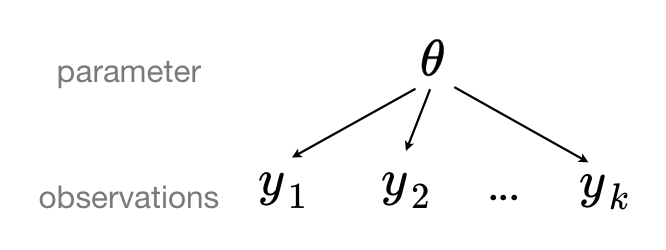
\includegraphics{images/pooled.png}
\caption{image}
\end{figure}

\hypertarget{unpooled-model}{%
\subsubsection{Unpooled Model}\label{unpooled-model}}

In a completely unpooled model, each group (airline) in this case is
treated independently.

\begin{figure}
\centering
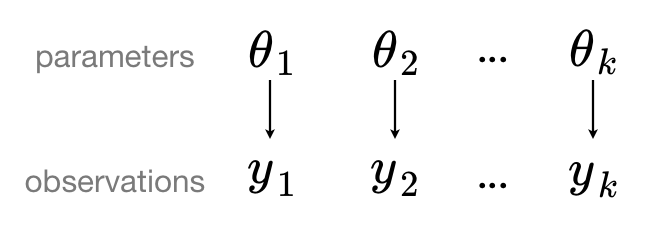
\includegraphics{images/unpooled.png}
\caption{image}
\end{figure}

\hypertarget{hierarchical-model}{%
\subsubsection{Hierarchical Model}\label{hierarchical-model}}

In a hierarchical model, the parameters come from a population
distribution, which means they are neither completely the same, or
completely independent. This allows us to use all observations as well
as grouped observations to compute the model parameters.

\begin{figure}
\centering
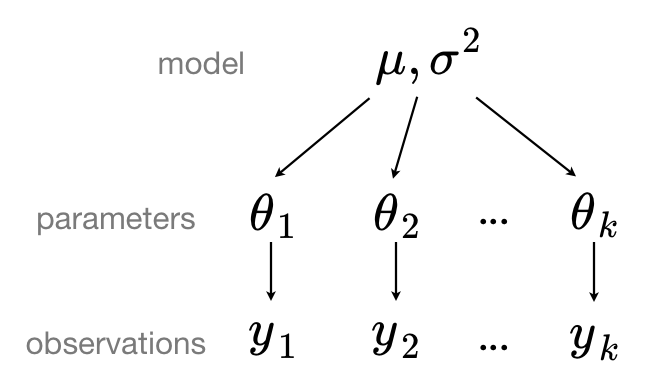
\includegraphics{images/hierarchical.png}
\caption{image}
\end{figure}

The overall objective of this notebook is to create several hierarchical
regression models. We want to find the relationship between the
departure delay in minutes and the arrival delay in minutes. My
hypothesis is that this should be close to 1, however, some airlines may
be better at making up time ``in the air''. If the slope is less than
one between departure delay and arrival delay, that means the flight has
made up time while on-route. Perhaps some airlines have a much smaller
slope indicating they are consistently better at making up time. We can
also use the intercept to model the arrival delay given no departure
delay. This might also be useful to compare between airlines.

    \begin{Verbatim}[commandchars=\\\{\}]
{\color{incolor}In [{\color{incolor}1}]:} \PY{k+kn}{import} \PY{n+nn}{numpy} \PY{k}{as} \PY{n+nn}{np}
        \PY{k+kn}{import} \PY{n+nn}{pandas} \PY{k}{as} \PY{n+nn}{pd}
        
        \PY{k+kn}{import} \PY{n+nn}{matplotlib}\PY{n+nn}{.}\PY{n+nn}{pyplot} \PY{k}{as} \PY{n+nn}{plt}
        \PY{k+kn}{import} \PY{n+nn}{matplotlib} 
        
        \PY{k+kn}{from} \PY{n+nn}{IPython}\PY{n+nn}{.}\PY{n+nn}{core}\PY{n+nn}{.}\PY{n+nn}{pylabtools} \PY{k}{import} \PY{n}{figsize}
        \PY{k+kn}{import} \PY{n+nn}{seaborn} \PY{k}{as} \PY{n+nn}{sns}
        \PY{n}{sns}\PY{o}{.}\PY{n}{set\PYZus{}context}\PY{p}{(}\PY{l+s+s1}{\PYZsq{}}\PY{l+s+s1}{poster}\PY{l+s+s1}{\PYZsq{}}\PY{p}{)}
        
        \PY{o}{\PYZpc{}}\PY{k}{matplotlib} inline
        
        \PY{k+kn}{import} \PY{n+nn}{pymc3} \PY{k}{as} \PY{n+nn}{pm}
        
        \PY{k+kn}{import} \PY{n+nn}{scipy}
\end{Verbatim}


    \begin{Verbatim}[commandchars=\\\{\}]
WARNING (theano.tensor.blas): Using NumPy C-API based implementation for BLAS functions.

    \end{Verbatim}

    \hypertarget{data-exploration}{%
\section{Data Exploration}\label{data-exploration}}

First we will read in the data and look at the distributions of
departure delays and arrival delays. The units are in minutes, and a
negative measurement means the flight was early. I will remove the
extreme outlying points, those delays longer than 200 minutes. This is
so we can approximate the arrival and departure delay times as a normal
distribution. Another option would be to take the log of the delays to
normalize them.

    \begin{Verbatim}[commandchars=\\\{\}]
{\color{incolor}In [{\color{incolor}2}]:} \PY{n}{flights} \PY{o}{=} \PY{n}{pd}\PY{o}{.}\PY{n}{read\PYZus{}csv}\PY{p}{(}\PY{l+s+s1}{\PYZsq{}}\PY{l+s+s1}{data/flights.csv}\PY{l+s+s1}{\PYZsq{}}\PY{p}{,} \PY{n}{index\PYZus{}col}\PY{o}{=}\PY{l+m+mi}{0}\PY{p}{)}
        \PY{n}{flights}\PY{o}{.}\PY{n}{dropna}\PY{p}{(}\PY{n}{subset}\PY{o}{=}\PY{p}{[}\PY{l+s+s1}{\PYZsq{}}\PY{l+s+s1}{dep\PYZus{}delay}\PY{l+s+s1}{\PYZsq{}}\PY{p}{,} \PY{l+s+s1}{\PYZsq{}}\PY{l+s+s1}{arr\PYZus{}delay}\PY{l+s+s1}{\PYZsq{}}\PY{p}{]}\PY{p}{,} \PY{n}{inplace}\PY{o}{=}\PY{k+kc}{True}\PY{p}{)}
        
        
        \PY{n}{carriers} \PY{o}{=} \PY{n}{pd}\PY{o}{.}\PY{n}{read\PYZus{}csv}\PY{p}{(}\PY{l+s+s1}{\PYZsq{}}\PY{l+s+s1}{data/airlines.csv}\PY{l+s+s1}{\PYZsq{}}\PY{p}{)}
        \PY{n}{flights} \PY{o}{=} \PY{n}{flights}\PY{o}{.}\PY{n}{merge}\PY{p}{(}\PY{n}{carriers}\PY{p}{,} \PY{n}{how} \PY{o}{=} \PY{l+s+s1}{\PYZsq{}}\PY{l+s+s1}{left}\PY{l+s+s1}{\PYZsq{}}\PY{p}{,} \PY{n}{on} \PY{o}{=} \PY{l+s+s1}{\PYZsq{}}\PY{l+s+s1}{carrier}\PY{l+s+s1}{\PYZsq{}} \PY{p}{)}
        \PY{n}{flights}\PY{p}{[}\PY{l+s+s1}{\PYZsq{}}\PY{l+s+s1}{carrier}\PY{l+s+s1}{\PYZsq{}}\PY{p}{]} \PY{o}{=} \PY{n}{flights}\PY{p}{[}\PY{l+s+s1}{\PYZsq{}}\PY{l+s+s1}{name}\PY{l+s+s1}{\PYZsq{}}\PY{p}{]}
        \PY{n}{flights}\PY{o}{.}\PY{n}{drop}\PY{p}{(}\PY{n}{columns}\PY{o}{=}\PY{l+s+s1}{\PYZsq{}}\PY{l+s+s1}{name}\PY{l+s+s1}{\PYZsq{}}\PY{p}{,} \PY{n}{inplace}\PY{o}{=}\PY{k+kc}{True}\PY{p}{)}
        
        \PY{n}{flights} \PY{o}{=} \PY{n}{flights}\PY{p}{[}\PY{p}{(}\PY{n}{flights}\PY{o}{.}\PY{n}{dep\PYZus{}delay} \PY{o}{\PYZlt{}} \PY{l+m+mi}{200}\PY{p}{)} \PY{o}{\PYZam{}} \PY{p}{(}\PY{n}{flights}\PY{o}{.}\PY{n}{arr\PYZus{}delay} \PY{o}{\PYZlt{}} \PY{l+m+mi}{200}\PY{p}{)}\PY{p}{]}
        \PY{n}{flights\PYZus{}subset} \PY{o}{=} \PY{n}{flights}\PY{p}{[}\PY{p}{[}\PY{l+s+s1}{\PYZsq{}}\PY{l+s+s1}{carrier}\PY{l+s+s1}{\PYZsq{}}\PY{p}{,} \PY{l+s+s1}{\PYZsq{}}\PY{l+s+s1}{dep\PYZus{}delay}\PY{l+s+s1}{\PYZsq{}}\PY{p}{,} \PY{l+s+s1}{\PYZsq{}}\PY{l+s+s1}{arr\PYZus{}delay}\PY{l+s+s1}{\PYZsq{}}\PY{p}{]}\PY{p}{]}
        \PY{n}{flights\PYZus{}melted} \PY{o}{=} \PY{n}{flights\PYZus{}subset}\PY{o}{.}\PY{n}{melt}\PY{p}{(}\PY{n}{id\PYZus{}vars}\PY{o}{=}\PY{l+s+s1}{\PYZsq{}}\PY{l+s+s1}{carrier}\PY{l+s+s1}{\PYZsq{}}\PY{p}{,} \PY{n}{value\PYZus{}name}\PY{o}{=}\PY{l+s+s1}{\PYZsq{}}\PY{l+s+s1}{value}\PY{l+s+s1}{\PYZsq{}}\PY{p}{,} \PY{n}{var\PYZus{}name}\PY{o}{=}\PY{l+s+s1}{\PYZsq{}}\PY{l+s+s1}{type}\PY{l+s+s1}{\PYZsq{}}\PY{p}{)}
        
        \PY{n}{figsize}\PY{p}{(}\PY{l+m+mi}{16}\PY{p}{,} \PY{l+m+mi}{8}\PY{p}{)}
        \PY{n}{grid} \PY{o}{=} \PY{n}{sns}\PY{o}{.}\PY{n}{FacetGrid}\PY{p}{(}\PY{n}{flights\PYZus{}melted}\PY{p}{,} \PY{n}{col} \PY{o}{=} \PY{l+s+s1}{\PYZsq{}}\PY{l+s+s1}{type}\PY{l+s+s1}{\PYZsq{}}\PY{p}{,} \PY{n}{hue} \PY{o}{=} \PY{l+s+s1}{\PYZsq{}}\PY{l+s+s1}{carrier}\PY{l+s+s1}{\PYZsq{}}\PY{p}{,} \PY{n}{size}\PY{o}{=}\PY{l+m+mi}{8}\PY{p}{,} \PY{n}{sharey}\PY{o}{=}\PY{k+kc}{False}\PY{p}{)}
        \PY{n}{grid}\PY{o}{.}\PY{n}{map}\PY{p}{(}\PY{n}{sns}\PY{o}{.}\PY{n}{kdeplot}\PY{p}{,} \PY{l+s+s1}{\PYZsq{}}\PY{l+s+s1}{value}\PY{l+s+s1}{\PYZsq{}}\PY{p}{)}
        \PY{n}{grid}\PY{o}{.}\PY{n}{add\PYZus{}legend}\PY{p}{(}\PY{p}{)}\PY{p}{;}
        \PY{n}{ax1} \PY{o}{=} \PY{n}{grid}\PY{o}{.}\PY{n}{axes}\PY{p}{[}\PY{l+m+mi}{0}\PY{p}{]}\PY{p}{[}\PY{l+m+mi}{0}\PY{p}{]}
        \PY{n}{ax1}\PY{o}{.}\PY{n}{set\PYZus{}xlabel}\PY{p}{(}\PY{l+s+s1}{\PYZsq{}}\PY{l+s+s1}{Dep Delay in Minutes}\PY{l+s+s1}{\PYZsq{}}\PY{p}{)}
        \PY{n}{ax1}\PY{o}{.}\PY{n}{set\PYZus{}title}\PY{p}{(}\PY{l+s+s1}{\PYZsq{}}\PY{l+s+s1}{Departure Delay}\PY{l+s+s1}{\PYZsq{}}\PY{p}{)}
        
        \PY{n}{ax2} \PY{o}{=} \PY{n}{grid}\PY{o}{.}\PY{n}{axes}\PY{p}{[}\PY{l+m+mi}{0}\PY{p}{]}\PY{p}{[}\PY{l+m+mi}{1}\PY{p}{]}
        \PY{n}{ax2}\PY{o}{.}\PY{n}{set\PYZus{}xlabel}\PY{p}{(}\PY{l+s+s1}{\PYZsq{}}\PY{l+s+s1}{Arr Delay in Minutes}\PY{l+s+s1}{\PYZsq{}}\PY{p}{)}
        \PY{n}{ax2}\PY{o}{.}\PY{n}{set\PYZus{}title}\PY{p}{(}\PY{l+s+s1}{\PYZsq{}}\PY{l+s+s1}{Arrival Delay}\PY{l+s+s1}{\PYZsq{}}\PY{p}{)}\PY{p}{;}
        \PY{n}{ax1}\PY{o}{.}\PY{n}{set\PYZus{}ylabel}\PY{p}{(}\PY{l+s+s1}{\PYZsq{}}\PY{l+s+s1}{Density Estimate}\PY{l+s+s1}{\PYZsq{}}\PY{p}{)}\PY{p}{;}
\end{Verbatim}


    \begin{center}
    \adjustimage{max size={0.9\linewidth}{0.9\paperheight}}{output_3_0.png}
    \end{center}
    { \hspace*{\fill} \\}
    
    The delays are approximately normal. This will simplify the modeling
allow we could also used a skewed normal because the distributions have
a rightward, or positive skew.

    \begin{Verbatim}[commandchars=\\\{\}]
{\color{incolor}In [{\color{incolor}3}]:} \PY{n}{sns}\PY{o}{.}\PY{n}{lmplot}\PY{p}{(}\PY{l+s+s1}{\PYZsq{}}\PY{l+s+s1}{dep\PYZus{}delay}\PY{l+s+s1}{\PYZsq{}}\PY{p}{,} \PY{l+s+s1}{\PYZsq{}}\PY{l+s+s1}{arr\PYZus{}delay}\PY{l+s+s1}{\PYZsq{}}\PY{p}{,} \PY{n}{flights}\PY{p}{,} 
                   \PY{n}{fit\PYZus{}reg} \PY{o}{=} \PY{k+kc}{False}\PY{p}{,} \PY{n}{hue} \PY{o}{=} \PY{l+s+s1}{\PYZsq{}}\PY{l+s+s1}{carrier}\PY{l+s+s1}{\PYZsq{}}\PY{p}{,} \PY{n}{size} \PY{o}{=} \PY{l+m+mi}{8}\PY{p}{)}\PY{p}{;}
        \PY{n}{plt}\PY{o}{.}\PY{n}{title}\PY{p}{(}\PY{l+s+s1}{\PYZsq{}}\PY{l+s+s1}{Arrival Delay vs. Departure Delay}\PY{l+s+s1}{\PYZsq{}}\PY{p}{)}\PY{p}{;}
\end{Verbatim}


    \begin{center}
    \adjustimage{max size={0.9\linewidth}{0.9\paperheight}}{output_5_0.png}
    \end{center}
    { \hspace*{\fill} \\}
    
    The relationship between departure and arrival delay looks to be nearly
1:1.

    \begin{Verbatim}[commandchars=\\\{\}]
{\color{incolor}In [{\color{incolor}4}]:} \PY{c+c1}{\PYZsh{} Restrict to first 10000 flights }
        \PY{n}{flights} \PY{o}{=} \PY{n}{flights}\PY{o}{.}\PY{n}{sample}\PY{p}{(}\PY{n}{frac}\PY{o}{=}\PY{l+m+mi}{1}\PY{p}{,} \PY{n}{random\PYZus{}state}\PY{o}{=}\PY{l+m+mi}{50}\PY{p}{)}\PY{p}{[}\PY{p}{:}\PY{l+m+mi}{10000}\PY{p}{]}
        
        \PY{c+c1}{\PYZsh{} Create carrier look up dict and list of codes}
        \PY{n}{carriers} \PY{o}{=} \PY{n}{flights}\PY{p}{[}\PY{l+s+s1}{\PYZsq{}}\PY{l+s+s1}{carrier}\PY{l+s+s1}{\PYZsq{}}\PY{p}{]}\PY{o}{.}\PY{n}{unique}\PY{p}{(}\PY{p}{)}
        \PY{n}{carrier\PYZus{}lookup} \PY{o}{=} \PY{n+nb}{dict}\PY{p}{(}\PY{n+nb}{zip}\PY{p}{(}\PY{n}{carriers}\PY{p}{,} \PY{n+nb}{range}\PY{p}{(}\PY{n+nb}{len}\PY{p}{(}\PY{n}{carriers}\PY{p}{)}\PY{p}{)}\PY{p}{)}\PY{p}{)}
        \PY{n}{carrier\PYZus{}codes} \PY{o}{=} \PY{n}{flights}\PY{p}{[}\PY{l+s+s1}{\PYZsq{}}\PY{l+s+s1}{carrier\PYZus{}code}\PY{l+s+s1}{\PYZsq{}}\PY{p}{]} \PY{o}{=} \PY{n}{flights}\PY{p}{[}\PY{l+s+s1}{\PYZsq{}}\PY{l+s+s1}{carrier}\PY{l+s+s1}{\PYZsq{}}\PY{p}{]}\PY{o}{.}\PY{n}{replace}\PY{p}{(}\PY{n}{carrier\PYZus{}lookup}\PY{p}{)}\PY{o}{.}\PY{n}{values}
\end{Verbatim}


    \hypertarget{pooled-model-for-flight-delay}{%
\section{Pooled Model for Flight
Delay}\label{pooled-model-for-flight-delay}}

The first model will consider all of the flights together. This is a
linear regression, so we are trying to find the slope of the
relationship between arrival delay and departure delay. We will also
find the intercept, which in this problem represents the arrival delay
with no departure delay.

    \begin{Verbatim}[commandchars=\\\{\}]
{\color{incolor}In [{\color{incolor}5}]:} \PY{n}{dep} \PY{o}{=} \PY{n}{np}\PY{o}{.}\PY{n}{array}\PY{p}{(}\PY{n}{flights}\PY{p}{[}\PY{l+s+s1}{\PYZsq{}}\PY{l+s+s1}{dep\PYZus{}delay}\PY{l+s+s1}{\PYZsq{}}\PY{p}{]}\PY{o}{.}\PY{n}{values}\PY{p}{)}
        \PY{n}{arr} \PY{o}{=} \PY{n}{np}\PY{o}{.}\PY{n}{array}\PY{p}{(}\PY{n}{flights}\PY{p}{[}\PY{l+s+s1}{\PYZsq{}}\PY{l+s+s1}{arr\PYZus{}delay}\PY{l+s+s1}{\PYZsq{}}\PY{p}{]}\PY{o}{.}\PY{n}{values}\PY{p}{)}
\end{Verbatim}


    We will approximate the arrival and departure delays as normal
distributions.

    \begin{Verbatim}[commandchars=\\\{\}]
{\color{incolor}In [{\color{incolor}6}]:} \PY{n}{plt}\PY{o}{.}\PY{n}{figure}\PY{p}{(}\PY{n}{figsize}\PY{o}{=}\PY{p}{(}\PY{l+m+mi}{8}\PY{p}{,} \PY{l+m+mi}{6}\PY{p}{)}\PY{p}{)}
        \PY{n}{sns}\PY{o}{.}\PY{n}{distplot}\PY{p}{(}\PY{n}{arr}\PY{p}{,} \PY{n}{color} \PY{o}{=} \PY{l+s+s1}{\PYZsq{}}\PY{l+s+s1}{darkgreen}\PY{l+s+s1}{\PYZsq{}}\PY{p}{)}
        \PY{n}{plt}\PY{o}{.}\PY{n}{title}\PY{p}{(}\PY{l+s+s1}{\PYZsq{}}\PY{l+s+s1}{Arrival Delay Distribution}\PY{l+s+s1}{\PYZsq{}}\PY{p}{)}\PY{p}{;}
        \PY{n}{plt}\PY{o}{.}\PY{n}{xlabel}\PY{p}{(}\PY{l+s+s1}{\PYZsq{}}\PY{l+s+s1}{Delay in minutes}\PY{l+s+s1}{\PYZsq{}}\PY{p}{)}\PY{p}{;} \PY{n}{plt}\PY{o}{.}\PY{n}{ylabel}\PY{p}{(}\PY{l+s+s1}{\PYZsq{}}\PY{l+s+s1}{Density}\PY{l+s+s1}{\PYZsq{}}\PY{p}{)}\PY{p}{;}
\end{Verbatim}


    \begin{center}
    \adjustimage{max size={0.9\linewidth}{0.9\paperheight}}{output_11_0.png}
    \end{center}
    { \hspace*{\fill} \\}
    
    \begin{Verbatim}[commandchars=\\\{\}]
{\color{incolor}In [{\color{incolor}7}]:} \PY{n}{plt}\PY{o}{.}\PY{n}{figure}\PY{p}{(}\PY{n}{figsize}\PY{o}{=}\PY{p}{(}\PY{l+m+mi}{8}\PY{p}{,} \PY{l+m+mi}{6}\PY{p}{)}\PY{p}{)}
        \PY{n}{sns}\PY{o}{.}\PY{n}{distplot}\PY{p}{(}\PY{n}{dep}\PY{p}{,} \PY{n}{color} \PY{o}{=} \PY{l+s+s1}{\PYZsq{}}\PY{l+s+s1}{darkgreen}\PY{l+s+s1}{\PYZsq{}}\PY{p}{)}
        \PY{n}{plt}\PY{o}{.}\PY{n}{title}\PY{p}{(}\PY{l+s+s1}{\PYZsq{}}\PY{l+s+s1}{Departure Delay Distribution}\PY{l+s+s1}{\PYZsq{}}\PY{p}{)}\PY{p}{;}
        \PY{n}{plt}\PY{o}{.}\PY{n}{xlabel}\PY{p}{(}\PY{l+s+s1}{\PYZsq{}}\PY{l+s+s1}{Delay in minutes}\PY{l+s+s1}{\PYZsq{}}\PY{p}{)}\PY{p}{;} \PY{n}{plt}\PY{o}{.}\PY{n}{ylabel}\PY{p}{(}\PY{l+s+s1}{\PYZsq{}}\PY{l+s+s1}{Density}\PY{l+s+s1}{\PYZsq{}}\PY{p}{)}\PY{p}{;}
\end{Verbatim}


    \begin{center}
    \adjustimage{max size={0.9\linewidth}{0.9\paperheight}}{output_12_0.png}
    \end{center}
    { \hspace*{\fill} \\}
    
    \begin{Verbatim}[commandchars=\\\{\}]
{\color{incolor}In [{\color{incolor}8}]:} \PY{n}{plt}\PY{o}{.}\PY{n}{figure}\PY{p}{(}\PY{n}{figsize}\PY{o}{=}\PY{p}{(}\PY{l+m+mi}{8}\PY{p}{,} \PY{l+m+mi}{6}\PY{p}{)}\PY{p}{)}
        \PY{n}{x} \PY{o}{=} \PY{n}{np}\PY{o}{.}\PY{n}{linspace}\PY{p}{(}\PY{n+nb}{min}\PY{p}{(}\PY{n}{arr}\PY{p}{)}\PY{p}{,} \PY{n+nb}{max}\PY{p}{(}\PY{n}{arr}\PY{p}{)}\PY{p}{)}
        \PY{n}{y} \PY{o}{=} \PY{n}{scipy}\PY{o}{.}\PY{n}{stats}\PY{o}{.}\PY{n}{norm}\PY{o}{.}\PY{n}{pdf}\PY{p}{(}\PY{n}{x}\PY{p}{,} \PY{n}{loc} \PY{o}{=} \PY{n}{np}\PY{o}{.}\PY{n}{mean}\PY{p}{(}\PY{n}{arr}\PY{p}{)}\PY{p}{,}\PY{n}{scale} \PY{o}{=} \PY{n}{np}\PY{o}{.}\PY{n}{std}\PY{p}{(}\PY{n}{arr}\PY{p}{)}\PY{p}{)}
        \PY{n}{plt}\PY{o}{.}\PY{n}{plot}\PY{p}{(}\PY{n}{x}\PY{p}{,} \PY{n}{y}\PY{p}{)}\PY{p}{;}
        \PY{n}{plt}\PY{o}{.}\PY{n}{title}\PY{p}{(}\PY{l+s+s1}{\PYZsq{}}\PY{l+s+s1}{Normal Distribution for Arrivals}\PY{l+s+s1}{\PYZsq{}}\PY{p}{)}
        \PY{n}{plt}\PY{o}{.}\PY{n}{ylabel}\PY{p}{(}\PY{l+s+s1}{\PYZsq{}}\PY{l+s+s1}{Density}\PY{l+s+s1}{\PYZsq{}}\PY{p}{)}\PY{p}{;}
\end{Verbatim}


    \begin{center}
    \adjustimage{max size={0.9\linewidth}{0.9\paperheight}}{output_13_0.png}
    \end{center}
    { \hspace*{\fill} \\}
    
    \begin{Verbatim}[commandchars=\\\{\}]
{\color{incolor}In [{\color{incolor}9}]:} \PY{n}{plt}\PY{o}{.}\PY{n}{figure}\PY{p}{(}\PY{n}{figsize}\PY{o}{=}\PY{p}{(}\PY{l+m+mi}{8}\PY{p}{,} \PY{l+m+mi}{6}\PY{p}{)}\PY{p}{)}
        \PY{n}{x} \PY{o}{=} \PY{n}{np}\PY{o}{.}\PY{n}{linspace}\PY{p}{(}\PY{n+nb}{min}\PY{p}{(}\PY{n}{dep}\PY{p}{)}\PY{p}{,} \PY{n+nb}{max}\PY{p}{(}\PY{n}{dep}\PY{p}{)}\PY{p}{)}
        \PY{n}{y} \PY{o}{=} \PY{n}{scipy}\PY{o}{.}\PY{n}{stats}\PY{o}{.}\PY{n}{norm}\PY{o}{.}\PY{n}{pdf}\PY{p}{(}\PY{n}{x}\PY{p}{,} \PY{n}{loc} \PY{o}{=} \PY{n}{np}\PY{o}{.}\PY{n}{mean}\PY{p}{(}\PY{n}{dep}\PY{p}{)}\PY{p}{,}\PY{n}{scale} \PY{o}{=} \PY{n}{np}\PY{o}{.}\PY{n}{std}\PY{p}{(}\PY{n}{dep}\PY{p}{)}\PY{p}{)}
        \PY{n}{plt}\PY{o}{.}\PY{n}{plot}\PY{p}{(}\PY{n}{x}\PY{p}{,} \PY{n}{y}\PY{p}{)}\PY{p}{;}
        \PY{n}{plt}\PY{o}{.}\PY{n}{title}\PY{p}{(}\PY{l+s+s1}{\PYZsq{}}\PY{l+s+s1}{Normal Distribution for Departures}\PY{l+s+s1}{\PYZsq{}}\PY{p}{)}
        \PY{n}{plt}\PY{o}{.}\PY{n}{ylabel}\PY{p}{(}\PY{l+s+s1}{\PYZsq{}}\PY{l+s+s1}{Density}\PY{l+s+s1}{\PYZsq{}}\PY{p}{)}\PY{p}{;}
\end{Verbatim}


    \begin{center}
    \adjustimage{max size={0.9\linewidth}{0.9\paperheight}}{output_14_0.png}
    \end{center}
    { \hspace*{\fill} \\}
    
    \begin{Verbatim}[commandchars=\\\{\}]
{\color{incolor}In [{\color{incolor}10}]:} \PY{n+nb}{print}\PY{p}{(}\PY{l+s+s1}{\PYZsq{}}\PY{l+s+s1}{Correlation between departure delay and arrival delay: }\PY{l+s+si}{\PYZob{}:.4f\PYZcb{}}\PY{l+s+s1}{.}\PY{l+s+s1}{\PYZsq{}}\PY{o}{.}
               \PY{n+nb}{format}\PY{p}{(}\PY{n}{np}\PY{o}{.}\PY{n}{corrcoef}\PY{p}{(}\PY{n}{arr}\PY{p}{,} \PY{n}{dep}\PY{p}{)}\PY{p}{[}\PY{l+m+mi}{0}\PY{p}{]}\PY{p}{[}\PY{l+m+mi}{1}\PY{p}{]}\PY{p}{)}\PY{p}{)}
         \PY{n+nb}{print}\PY{p}{(}\PY{l+s+s1}{\PYZsq{}}\PY{l+s+s1}{Skew of Arrival Delay: }\PY{l+s+si}{\PYZob{}:.4f\PYZcb{}}\PY{l+s+s1}{.}\PY{l+s+s1}{\PYZsq{}}\PY{o}{.}\PY{n}{format}\PY{p}{(}\PY{n}{scipy}\PY{o}{.}\PY{n}{stats}\PY{o}{.}\PY{n}{skew}\PY{p}{(}\PY{n}{arr}\PY{p}{)}\PY{p}{)}\PY{p}{)}
         \PY{n+nb}{print}\PY{p}{(}\PY{l+s+s1}{\PYZsq{}}\PY{l+s+s1}{Average Delay Time: }\PY{l+s+si}{\PYZob{}:.4f\PYZcb{}}\PY{l+s+s1}{ minutes.}\PY{l+s+s1}{\PYZsq{}}\PY{o}{.}\PY{n}{format}\PY{p}{(}\PY{n}{np}\PY{o}{.}\PY{n}{mean}\PY{p}{(}\PY{n}{arr}\PY{p}{)}\PY{p}{)}\PY{p}{)}
\end{Verbatim}


    \begin{Verbatim}[commandchars=\\\{\}]
Correlation between departure delay and arrival delay: 0.8631.
Skew of Arrival Delay: 2.0803.
Average Delay Time: 3.7169 minutes.

    \end{Verbatim}

    The pooled model treats all flights as coming from the same
distribution. We estimate one slope and one intercept for all of the
flights regardless of carrier. The equation for this model is
\[y_i = \alpha + \beta x_i + \epsilon_i\]

Where we have an intercept, slope (relationship between the arrival and
departure delay) and a model error.

    \begin{Verbatim}[commandchars=\\\{\}]
{\color{incolor}In [{\color{incolor}11}]:} \PY{c+c1}{\PYZsh{} Treat all of observations as coming from same distribution}
         \PY{k}{with} \PY{n}{pm}\PY{o}{.}\PY{n}{Model}\PY{p}{(}\PY{p}{)} \PY{k}{as} \PY{n}{pooled\PYZus{}model}\PY{p}{:}
             
             \PY{c+c1}{\PYZsh{} Beta is vector of model parameters: [intercept, slope]}
             \PY{n}{beta} \PY{o}{=} \PY{n}{pm}\PY{o}{.}\PY{n}{Normal}\PY{p}{(}\PY{l+s+s1}{\PYZsq{}}\PY{l+s+s1}{beta}\PY{l+s+s1}{\PYZsq{}}\PY{p}{,} \PY{n}{testval} \PY{o}{=} \PY{p}{[}\PY{l+m+mi}{0}\PY{p}{,} \PY{n}{np}\PY{o}{.}\PY{n}{corrcoef}\PY{p}{(}\PY{n}{arr}\PY{p}{,} \PY{n}{dep}\PY{p}{)}\PY{p}{[}\PY{l+m+mi}{0}\PY{p}{]}\PY{p}{[}\PY{l+m+mi}{1}\PY{p}{]}\PY{p}{]}\PY{p}{,}
                              \PY{n}{mu} \PY{o}{=} \PY{l+m+mi}{0}\PY{p}{,} \PY{n}{sd} \PY{o}{=} \PY{l+m+mi}{10}\PY{p}{,} \PY{n}{shape}\PY{o}{=}\PY{l+m+mi}{2}\PY{p}{)}
             
             \PY{c+c1}{\PYZsh{} Sigma is standard deviation of observations}
             \PY{n}{sigma} \PY{o}{=} \PY{n}{pm}\PY{o}{.}\PY{n}{HalfCauchy}\PY{p}{(}\PY{l+s+s1}{\PYZsq{}}\PY{l+s+s1}{sigma}\PY{l+s+s1}{\PYZsq{}}\PY{p}{,} \PY{l+m+mi}{5}\PY{p}{)}
             
             \PY{c+c1}{\PYZsh{} Linear equation for the arrival delay based on departure delay}
             \PY{n}{theta} \PY{o}{=} \PY{n}{beta}\PY{p}{[}\PY{l+m+mi}{0}\PY{p}{]} \PY{o}{+} \PY{n}{beta}\PY{p}{[}\PY{l+m+mi}{1}\PY{p}{]} \PY{o}{*} \PY{n}{dep}
             
             \PY{c+c1}{\PYZsh{} The arrival delays are assumed to be normally distributed}
             \PY{n}{y} \PY{o}{=} \PY{n}{pm}\PY{o}{.}\PY{n}{Normal}\PY{p}{(}\PY{l+s+s1}{\PYZsq{}}\PY{l+s+s1}{y}\PY{l+s+s1}{\PYZsq{}}\PY{p}{,} \PY{n}{mu}\PY{o}{=}\PY{n}{theta}\PY{p}{,} \PY{n}{sd}\PY{o}{=}\PY{n}{sigma}\PY{p}{,} \PY{n}{observed}\PY{o}{=}\PY{n}{arr}\PY{p}{)}
             
             \PY{c+c1}{\PYZsh{} Trace from pooled model}
             \PY{n}{pooled\PYZus{}trace} \PY{o}{=} \PY{n}{pm}\PY{o}{.}\PY{n}{sample}\PY{p}{(}\PY{l+m+mi}{1000}\PY{p}{)}
\end{Verbatim}


    \begin{Verbatim}[commandchars=\\\{\}]
Auto-assigning NUTS sampler{\ldots}
Initializing NUTS using jitter+adapt\_diag{\ldots}
Multiprocess sampling (2 chains in 2 jobs)
NUTS: [sigma\_log\_\_, beta]

    \end{Verbatim}

    \begin{Verbatim}[commandchars=\\\{\}]
{\color{incolor}In [{\color{incolor}12}]:} \PY{c+c1}{\PYZsh{} Intercept and slope are mean of traces}
         \PY{n}{pooled\PYZus{}intercept}\PY{p}{,} \PY{n}{pooled\PYZus{}slope} \PY{o}{=} \PY{n}{pooled\PYZus{}trace}\PY{p}{[}\PY{l+s+s1}{\PYZsq{}}\PY{l+s+s1}{beta}\PY{l+s+s1}{\PYZsq{}}\PY{p}{]}\PY{o}{.}\PY{n}{mean}\PY{p}{(}\PY{n}{axis}\PY{o}{=}\PY{l+m+mi}{0}\PY{p}{)}
         \PY{n}{pooled\PYZus{}sigma} \PY{o}{=} \PY{n}{pooled\PYZus{}trace}\PY{p}{[}\PY{l+s+s1}{\PYZsq{}}\PY{l+s+s1}{sigma}\PY{l+s+s1}{\PYZsq{}}\PY{p}{]}\PY{o}{.}\PY{n}{mean}\PY{p}{(}\PY{n}{axis}\PY{o}{=}\PY{l+m+mi}{0}\PY{p}{)}
\end{Verbatim}


    \begin{Verbatim}[commandchars=\\\{\}]
{\color{incolor}In [{\color{incolor}13}]:} \PY{n}{figsize}\PY{p}{(}\PY{l+m+mi}{10}\PY{p}{,} \PY{l+m+mi}{8}\PY{p}{)}
         
         \PY{c+c1}{\PYZsh{} Observations on a scatter plot}
         \PY{n}{plt}\PY{o}{.}\PY{n}{scatter}\PY{p}{(}\PY{n}{flights}\PY{p}{[}\PY{l+s+s1}{\PYZsq{}}\PY{l+s+s1}{dep\PYZus{}delay}\PY{l+s+s1}{\PYZsq{}}\PY{p}{]}\PY{p}{,} \PY{p}{(}\PY{n}{flights}\PY{p}{[}\PY{l+s+s1}{\PYZsq{}}\PY{l+s+s1}{arr\PYZus{}delay}\PY{l+s+s1}{\PYZsq{}}\PY{p}{]}\PY{p}{)}\PY{p}{,} \PY{n}{s} \PY{o}{=} \PY{l+m+mi}{50}\PY{p}{,} 
                    \PY{n}{alpha} \PY{o}{=} \PY{l+m+mf}{0.5}\PY{p}{,} \PY{n}{facecolor} \PY{o}{=} \PY{l+s+s1}{\PYZsq{}}\PY{l+s+s1}{b}\PY{l+s+s1}{\PYZsq{}}\PY{p}{,} \PY{n}{edgecolors} \PY{o}{=} \PY{l+s+s1}{\PYZsq{}}\PY{l+s+s1}{b}\PY{l+s+s1}{\PYZsq{}}\PY{p}{,} \PY{n}{label}\PY{o}{=}\PY{l+s+s1}{\PYZsq{}}\PY{l+s+s1}{obs}\PY{l+s+s1}{\PYZsq{}}\PY{p}{)}
         
         \PY{n}{xvals} \PY{o}{=} \PY{n}{np}\PY{o}{.}\PY{n}{linspace}\PY{p}{(}\PY{n+nb}{min}\PY{p}{(}\PY{n}{dep}\PY{p}{)}\PY{p}{,} \PY{n+nb}{max}\PY{p}{(}\PY{n}{dep}\PY{p}{)}\PY{p}{)}
         
         \PY{c+c1}{\PYZsh{} Line represents the model from sampling}
         \PY{n}{plt}\PY{o}{.}\PY{n}{plot}\PY{p}{(}\PY{n}{xvals}\PY{p}{,} \PY{n}{pooled\PYZus{}slope} \PY{o}{*} \PY{n}{xvals} \PY{o}{+} \PY{n}{pooled\PYZus{}intercept}\PY{p}{,} 
                  \PY{l+s+s1}{\PYZsq{}}\PY{l+s+s1}{r\PYZhy{}\PYZhy{}}\PY{l+s+s1}{\PYZsq{}}\PY{p}{,} \PY{n}{label} \PY{o}{=} \PY{l+s+s1}{\PYZsq{}}\PY{l+s+s1}{Pooled Model Estimate}\PY{l+s+s1}{\PYZsq{}}\PY{p}{)}\PY{p}{;}
         \PY{n}{plt}\PY{o}{.}\PY{n}{xlabel}\PY{p}{(}\PY{l+s+s1}{\PYZsq{}}\PY{l+s+s1}{Departure Delay}\PY{l+s+s1}{\PYZsq{}}\PY{p}{)}\PY{p}{;} \PY{n}{plt}\PY{o}{.}\PY{n}{ylabel}\PY{p}{(}\PY{l+s+s1}{\PYZsq{}}\PY{l+s+s1}{Arrival Delay}\PY{l+s+s1}{\PYZsq{}}\PY{p}{)}\PY{p}{;}
         \PY{n}{plt}\PY{o}{.}\PY{n}{legend}\PY{p}{(}\PY{n}{loc}\PY{o}{=}\PY{l+m+mi}{2}\PY{p}{)}\PY{p}{;}
         \PY{n}{plt}\PY{o}{.}\PY{n}{title}\PY{p}{(}\PY{l+s+s1}{\PYZsq{}}\PY{l+s+s1}{Observations and Pooled Model}\PY{l+s+s1}{\PYZsq{}}\PY{p}{)}\PY{p}{;}
\end{Verbatim}


    \begin{center}
    \adjustimage{max size={0.9\linewidth}{0.9\paperheight}}{output_19_0.png}
    \end{center}
    { \hspace*{\fill} \\}
    
    \begin{Verbatim}[commandchars=\\\{\}]
{\color{incolor}In [{\color{incolor}14}]:} \PY{n}{figsize}\PY{p}{(}\PY{l+m+mi}{8}\PY{p}{,} \PY{l+m+mi}{6}\PY{p}{)}
         \PY{n}{x} \PY{o}{=} \PY{n}{np}\PY{o}{.}\PY{n}{linspace}\PY{p}{(}\PY{n+nb}{min}\PY{p}{(}\PY{n}{arr}\PY{p}{)}\PY{p}{,} \PY{n+nb}{max}\PY{p}{(}\PY{n}{arr}\PY{p}{)}\PY{p}{)}
         \PY{n}{pooled\PYZus{}dist} \PY{o}{=} \PY{n}{scipy}\PY{o}{.}\PY{n}{stats}\PY{o}{.}\PY{n}{norm}\PY{o}{.}\PY{n}{pdf}\PY{p}{(}\PY{n}{x}\PY{p}{,} \PY{n}{loc} \PY{o}{=} \PY{n}{pooled\PYZus{}intercept}\PY{p}{,} 
                                               \PY{n}{scale} \PY{o}{=} \PY{n}{pooled\PYZus{}sigma}\PY{p}{)}
         \PY{n}{sns}\PY{o}{.}\PY{n}{kdeplot}\PY{p}{(}\PY{n}{arr}\PY{p}{)}
         \PY{n}{plt}\PY{o}{.}\PY{n}{plot}\PY{p}{(}\PY{n}{x}\PY{p}{,} \PY{n}{pooled\PYZus{}dist}\PY{p}{,} \PY{n}{label}\PY{o}{=}\PY{l+s+s1}{\PYZsq{}}\PY{l+s+s1}{model}\PY{l+s+s1}{\PYZsq{}}\PY{p}{)}
         \PY{n}{plt}\PY{o}{.}\PY{n}{legend}\PY{p}{(}\PY{p}{)}\PY{p}{;} \PY{n}{plt}\PY{o}{.}\PY{n}{xlabel}\PY{p}{(}\PY{l+s+s1}{\PYZsq{}}\PY{l+s+s1}{Delay in Minutes}\PY{l+s+s1}{\PYZsq{}}\PY{p}{)}\PY{p}{;}
         \PY{n}{plt}\PY{o}{.}\PY{n}{title}\PY{p}{(}\PY{l+s+s1}{\PYZsq{}}\PY{l+s+s1}{Pooled Distribution of Arrival Delays}\PY{l+s+s1}{\PYZsq{}}\PY{p}{)}\PY{p}{;}
\end{Verbatim}


    \begin{center}
    \adjustimage{max size={0.9\linewidth}{0.9\paperheight}}{output_20_0.png}
    \end{center}
    { \hspace*{\fill} \\}
    
    The complete pooling model aligns with all of the observations. Next, we
will move on to unpooled models and treating each carrier group
separately.

    \hypertarget{completely-unpooled-model}{%
\section{Completely Unpooled Model}\label{completely-unpooled-model}}

In the no pooling model, all groups are treated separately with no
dependence between the clusters. Each carrier will have its own slope
describing the relationship between the departure and arrival delay. The
equation for an unpooled model is:

\[y_i = \alpha_{j[i]} + \beta x_i + \epsilon_i\]

Where \(j = 1, \ldots, n\) for the number of carriers.

    \begin{Verbatim}[commandchars=\\\{\}]
{\color{incolor}In [{\color{incolor}15}]:} \PY{n}{carriers}
\end{Verbatim}


\begin{Verbatim}[commandchars=\\\{\}]
{\color{outcolor}Out[{\color{outcolor}15}]:} array(['Delta Air Lines Inc.', 'American Airlines Inc.',
                'Endeavor Air Inc.', 'United Air Lines Inc.',
                'ExpressJet Airlines Inc.', 'US Airways Inc.', 'JetBlue Airways',
                'Southwest Airlines Co.', 'Virgin America',
                'AirTran Airways Corporation', 'Envoy Air',
                'Frontier Airlines Inc.', 'Alaska Airlines Inc.',
                'Hawaiian Airlines Inc.', 'Mesa Airlines Inc.'], dtype=object)
\end{Verbatim}
            
    \begin{Verbatim}[commandchars=\\\{\}]
{\color{incolor}In [{\color{incolor}16}]:} \PY{k}{with} \PY{n}{pm}\PY{o}{.}\PY{n}{Model}\PY{p}{(}\PY{p}{)} \PY{k}{as} \PY{n}{unpooled\PYZus{}model}\PY{p}{:}
             
             \PY{c+c1}{\PYZsh{} Random Intercept}
             \PY{n}{beta0} \PY{o}{=} \PY{n}{pm}\PY{o}{.}\PY{n}{Normal}\PY{p}{(}\PY{l+s+s1}{\PYZsq{}}\PY{l+s+s1}{beta0}\PY{l+s+s1}{\PYZsq{}}\PY{p}{,} \PY{l+m+mi}{0}\PY{p}{,} \PY{n}{sd} \PY{o}{=} \PY{l+m+mi}{10}\PY{p}{,} \PY{n}{shape} \PY{o}{=} \PY{n+nb}{len}\PY{p}{(}\PY{n}{carriers}\PY{p}{)}\PY{p}{)}
             
             \PY{c+c1}{\PYZsh{} Slope}
             \PY{n}{beta1} \PY{o}{=} \PY{n}{pm}\PY{o}{.}\PY{n}{Normal}\PY{p}{(}\PY{l+s+s1}{\PYZsq{}}\PY{l+s+s1}{beta1}\PY{l+s+s1}{\PYZsq{}}\PY{p}{,} \PY{l+m+mi}{0}\PY{p}{,} \PY{n}{testval} \PY{o}{=} \PY{n}{np}\PY{o}{.}\PY{n}{corrcoef}\PY{p}{(}\PY{n}{arr}\PY{p}{,} \PY{n}{dep}\PY{p}{)}\PY{p}{[}\PY{l+m+mi}{0}\PY{p}{]}\PY{p}{[}\PY{l+m+mi}{1}\PY{p}{]}\PY{p}{,} \PY{n}{sd} \PY{o}{=} \PY{l+m+mi}{10}\PY{p}{)}
             
             \PY{c+c1}{\PYZsh{} Error for model}
             \PY{n}{sigma} \PY{o}{=} \PY{n}{pm}\PY{o}{.}\PY{n}{HalfCauchy}\PY{p}{(}\PY{l+s+s1}{\PYZsq{}}\PY{l+s+s1}{sigma}\PY{l+s+s1}{\PYZsq{}}\PY{p}{,} \PY{l+m+mi}{5}\PY{p}{)}
             
             \PY{c+c1}{\PYZsh{} Model}
             \PY{n}{theta} \PY{o}{=} \PY{n}{beta0}\PY{p}{[}\PY{n}{carrier\PYZus{}codes}\PY{p}{]} \PY{o}{+} \PY{n}{beta1} \PY{o}{*} \PY{n}{dep}
             
             \PY{c+c1}{\PYZsh{} Observations}
             \PY{n}{y} \PY{o}{=} \PY{n}{pm}\PY{o}{.}\PY{n}{Normal}\PY{p}{(}\PY{l+s+s1}{\PYZsq{}}\PY{l+s+s1}{y}\PY{l+s+s1}{\PYZsq{}}\PY{p}{,} \PY{n}{theta}\PY{p}{,} \PY{n}{sd} \PY{o}{=} \PY{n}{sigma}\PY{p}{,} \PY{n}{observed} \PY{o}{=} \PY{n}{arr}\PY{p}{)}
             \PY{n}{unpooled\PYZus{}trace} \PY{o}{=} \PY{n}{pm}\PY{o}{.}\PY{n}{sample}\PY{p}{(}\PY{l+m+mi}{1000}\PY{p}{)}
\end{Verbatim}


    \begin{Verbatim}[commandchars=\\\{\}]
Auto-assigning NUTS sampler{\ldots}
Initializing NUTS using jitter+adapt\_diag{\ldots}
Multiprocess sampling (2 chains in 2 jobs)
NUTS: [sigma\_log\_\_, beta1, beta0]

    \end{Verbatim}

    To visualize the unpooled model results, we can examine the intercepts
that were found for each airline. The slope is shared among the
airlines, but the intercepts are completely independent.

    \begin{Verbatim}[commandchars=\\\{\}]
{\color{incolor}In [{\color{incolor}17}]:} \PY{k+kn}{from} \PY{n+nn}{pymc3} \PY{k}{import} \PY{n}{forestplot}
         
         \PY{n}{figsize}\PY{p}{(}\PY{l+m+mi}{8}\PY{p}{,} \PY{l+m+mi}{12}\PY{p}{)}
         \PY{n}{forestplot}\PY{p}{(}\PY{n}{unpooled\PYZus{}trace}\PY{p}{,} \PY{n}{varnames}\PY{o}{=}\PY{p}{[}\PY{l+s+s1}{\PYZsq{}}\PY{l+s+s1}{beta0}\PY{l+s+s1}{\PYZsq{}}\PY{p}{]}\PY{p}{)}\PY{p}{;}
         \PY{n}{plt}\PY{o}{.}\PY{n}{suptitle}\PY{p}{(}\PY{l+s+s1}{\PYZsq{}}\PY{l+s+s1}{Distribution of Sampled Variables}\PY{l+s+s1}{\PYZsq{}}\PY{p}{)}\PY{p}{;}
\end{Verbatim}


    \begin{center}
    \adjustimage{max size={0.9\linewidth}{0.9\paperheight}}{output_26_0.png}
    \end{center}
    { \hspace*{\fill} \\}
    
    The intercepts differ by airline. The ``best'' airlines are those with
the lowest intercept which represents the arrival delay with no
departure delay. We can visualize this by ordering the airlines from the
lowest to the highest intercept.

    \begin{Verbatim}[commandchars=\\\{\}]
{\color{incolor}In [{\color{incolor}18}]:} \PY{n}{unpooled\PYZus{}estimates} \PY{o}{=} \PY{n}{pd}\PY{o}{.}\PY{n}{Series}\PY{p}{(}\PY{n}{unpooled\PYZus{}trace}\PY{p}{[}\PY{l+s+s1}{\PYZsq{}}\PY{l+s+s1}{beta0}\PY{l+s+s1}{\PYZsq{}}\PY{p}{]}\PY{o}{.}\PY{n}{mean}\PY{p}{(}\PY{n}{axis}\PY{o}{=}\PY{l+m+mi}{0}\PY{p}{)}\PY{p}{,} \PY{n}{index} \PY{o}{=} \PY{n}{carriers}\PY{p}{)}
         \PY{n}{unpooled\PYZus{}se} \PY{o}{=} \PY{n}{pd}\PY{o}{.}\PY{n}{Series}\PY{p}{(}\PY{n}{unpooled\PYZus{}trace}\PY{p}{[}\PY{l+s+s1}{\PYZsq{}}\PY{l+s+s1}{beta0}\PY{l+s+s1}{\PYZsq{}}\PY{p}{]}\PY{o}{.}\PY{n}{std}\PY{p}{(}\PY{n}{axis}\PY{o}{=}\PY{l+m+mi}{0}\PY{p}{)}\PY{p}{,} \PY{n}{index} \PY{o}{=} \PY{n}{carriers}\PY{p}{)}
\end{Verbatim}


    \begin{Verbatim}[commandchars=\\\{\}]
{\color{incolor}In [{\color{incolor}19}]:} \PY{n}{order} \PY{o}{=} \PY{n}{unpooled\PYZus{}estimates}\PY{o}{.}\PY{n}{sort\PYZus{}values}\PY{p}{(}\PY{p}{)}\PY{o}{.}\PY{n}{index}
         \PY{n}{figsize}\PY{p}{(}\PY{l+m+mi}{10}\PY{p}{,} \PY{l+m+mi}{8}\PY{p}{)}
         \PY{n}{plt}\PY{o}{.}\PY{n}{scatter}\PY{p}{(}\PY{n+nb}{range}\PY{p}{(}\PY{n+nb}{len}\PY{p}{(}\PY{n}{unpooled\PYZus{}estimates}\PY{p}{)}\PY{p}{)}\PY{p}{,} \PY{n}{unpooled\PYZus{}estimates}\PY{p}{[}\PY{n}{order}\PY{p}{]}\PY{p}{)}
         \PY{k}{for} \PY{n}{i}\PY{p}{,} \PY{n}{m}\PY{p}{,} \PY{n}{se} \PY{o+ow}{in} \PY{n+nb}{zip}\PY{p}{(}\PY{n+nb}{range}\PY{p}{(}\PY{n+nb}{len}\PY{p}{(}\PY{n}{unpooled\PYZus{}estimates}\PY{p}{)}\PY{p}{)}\PY{p}{,} \PY{n}{unpooled\PYZus{}estimates}\PY{p}{[}\PY{n}{order}\PY{p}{]}\PY{p}{,} \PY{n}{unpooled\PYZus{}se}\PY{p}{[}\PY{n}{order}\PY{p}{]}\PY{p}{)}\PY{p}{:}
             \PY{n}{plt}\PY{o}{.}\PY{n}{plot}\PY{p}{(}\PY{p}{[}\PY{n}{i}\PY{p}{,} \PY{n}{i}\PY{p}{]}\PY{p}{,} \PY{p}{[}\PY{n}{m} \PY{o}{\PYZhy{}} \PY{n}{se}\PY{p}{,} \PY{n}{m} \PY{o}{+} \PY{n}{se}\PY{p}{]}\PY{p}{,} \PY{l+s+s1}{\PYZsq{}}\PY{l+s+s1}{b\PYZhy{}}\PY{l+s+s1}{\PYZsq{}}\PY{p}{)}
             
         \PY{n}{plt}\PY{o}{.}\PY{n}{xticks}\PY{p}{(}\PY{n+nb}{range}\PY{p}{(}\PY{n+nb}{len}\PY{p}{(}\PY{n}{unpooled\PYZus{}estimates}\PY{p}{)}\PY{p}{)}\PY{p}{,} \PY{n}{order}\PY{p}{,} \PY{n}{rotation} \PY{o}{=} \PY{l+m+mi}{90}\PY{p}{)}\PY{p}{;}
         \PY{n}{plt}\PY{o}{.}\PY{n}{hlines}\PY{p}{(} \PY{n}{y} \PY{o}{=} \PY{n}{pooled\PYZus{}intercept}\PY{p}{,} \PY{n}{color} \PY{o}{=} \PY{l+s+s1}{\PYZsq{}}\PY{l+s+s1}{r}\PY{l+s+s1}{\PYZsq{}}\PY{p}{,} \PY{n}{linestyles}\PY{o}{=}\PY{l+s+s1}{\PYZsq{}}\PY{l+s+s1}{\PYZhy{}\PYZhy{}}\PY{l+s+s1}{\PYZsq{}}\PY{p}{,} \PY{n}{xmin} \PY{o}{=} \PY{l+m+mi}{0}\PY{p}{,} \PY{n}{xmax} \PY{o}{=} \PY{n+nb}{len}\PY{p}{(}\PY{n}{unpooled\PYZus{}estimates}\PY{p}{)}\PY{p}{)}
         \PY{n}{plt}\PY{o}{.}\PY{n}{text}\PY{p}{(}\PY{n}{x} \PY{o}{=} \PY{l+m+mi}{1}\PY{p}{,} \PY{n}{y} \PY{o}{=} \PY{n}{pooled\PYZus{}intercept} \PY{o}{+} \PY{o}{.}\PY{l+m+mi}{4}\PY{p}{,} \PY{n}{s} \PY{o}{=} \PY{l+s+s1}{\PYZsq{}}\PY{l+s+s1}{Pooled Intercept}\PY{l+s+s1}{\PYZsq{}}\PY{p}{)}
         \PY{n}{plt}\PY{o}{.}\PY{n}{xlabel}\PY{p}{(}\PY{l+s+s1}{\PYZsq{}}\PY{l+s+s1}{Carrier}\PY{l+s+s1}{\PYZsq{}}\PY{p}{)}\PY{p}{;} \PY{n}{plt}\PY{o}{.}\PY{n}{ylabel}\PY{p}{(}\PY{l+s+s1}{\PYZsq{}}\PY{l+s+s1}{Minutes}\PY{l+s+s1}{\PYZsq{}}\PY{p}{)}\PY{p}{;}
         \PY{n}{plt}\PY{o}{.}\PY{n}{title}\PY{p}{(}\PY{l+s+s1}{\PYZsq{}}\PY{l+s+s1}{Unpooled Estimate of Intercept}\PY{l+s+s1}{\PYZsq{}}\PY{p}{)}\PY{p}{;}
\end{Verbatim}


    \begin{center}
    \adjustimage{max size={0.9\linewidth}{0.9\paperheight}}{output_29_0.png}
    \end{center}
    { \hspace*{\fill} \\}
    
    Based on the unpooled model, Alaska Airlines is the best in terms of
arrival delays, and Frontier Arlines is the worse in terms of arrival
delays.

    We can also plot the pooled and unpooled models on the same graph for
several airlines. Airlines with unpooled estimates for the intercept
lower than the average are ``better'' because the intercept represents
the arrival delay with no departure delay.

    \begin{Verbatim}[commandchars=\\\{\}]
{\color{incolor}In [{\color{incolor}20}]:} \PY{n}{sample\PYZus{}airlines} \PY{o}{=} \PY{n+nb}{tuple}\PY{p}{(}\PY{n}{order}\PY{p}{[}\PY{p}{:}\PY{l+m+mi}{8}\PY{p}{]}\PY{p}{)}
         
         \PY{n}{fig}\PY{p}{,} \PY{n}{axes} \PY{o}{=} \PY{n}{plt}\PY{o}{.}\PY{n}{subplots}\PY{p}{(}\PY{l+m+mi}{2}\PY{p}{,} \PY{l+m+mi}{4}\PY{p}{,} \PY{n}{figsize}\PY{o}{=}\PY{p}{(}\PY{l+m+mi}{20}\PY{p}{,} \PY{l+m+mi}{14}\PY{p}{)}\PY{p}{,} \PY{n}{sharey}\PY{o}{=}\PY{k+kc}{True}\PY{p}{,} \PY{n}{sharex}\PY{o}{=}\PY{k+kc}{True}\PY{p}{)}
         \PY{n}{axes} \PY{o}{=} \PY{n}{axes}\PY{o}{.}\PY{n}{ravel}\PY{p}{(}\PY{p}{)}
         \PY{n}{m} \PY{o}{=} \PY{n}{unpooled\PYZus{}trace}\PY{p}{[}\PY{l+s+s1}{\PYZsq{}}\PY{l+s+s1}{beta1}\PY{l+s+s1}{\PYZsq{}}\PY{p}{]}\PY{o}{.}\PY{n}{mean}\PY{p}{(}\PY{p}{)}
         
         \PY{k}{for} \PY{n}{i}\PY{p}{,}\PY{n}{c} \PY{o+ow}{in} \PY{n+nb}{enumerate}\PY{p}{(}\PY{n}{sample\PYZus{}airlines}\PY{p}{)}\PY{p}{:}
             \PY{n}{y} \PY{o}{=} \PY{n}{flights}\PY{p}{[}\PY{l+s+s1}{\PYZsq{}}\PY{l+s+s1}{arr\PYZus{}delay}\PY{l+s+s1}{\PYZsq{}}\PY{p}{]}\PY{p}{[}\PY{n}{flights}\PY{p}{[}\PY{l+s+s1}{\PYZsq{}}\PY{l+s+s1}{carrier}\PY{l+s+s1}{\PYZsq{}}\PY{p}{]}\PY{o}{==}\PY{n}{c}\PY{p}{]}
             \PY{n}{x} \PY{o}{=} \PY{n}{flights}\PY{p}{[}\PY{l+s+s1}{\PYZsq{}}\PY{l+s+s1}{dep\PYZus{}delay}\PY{l+s+s1}{\PYZsq{}}\PY{p}{]}\PY{p}{[}\PY{n}{flights}\PY{p}{[}\PY{l+s+s1}{\PYZsq{}}\PY{l+s+s1}{carrier}\PY{l+s+s1}{\PYZsq{}}\PY{p}{]}\PY{o}{==}\PY{n}{c}\PY{p}{]}
             
             \PY{n}{axes}\PY{p}{[}\PY{n}{i}\PY{p}{]}\PY{o}{.}\PY{n}{scatter}\PY{p}{(}\PY{n}{x}\PY{p}{,} \PY{n}{y}\PY{p}{,} \PY{n}{alpha}\PY{o}{=}\PY{l+m+mf}{0.4}\PY{p}{,} \PY{n}{label} \PY{o}{=} \PY{l+s+s1}{\PYZsq{}}\PY{l+s+s1}{obs}\PY{l+s+s1}{\PYZsq{}}\PY{p}{)}
             
             \PY{c+c1}{\PYZsh{} No pooling model}
             \PY{n}{b} \PY{o}{=} \PY{n}{unpooled\PYZus{}estimates}\PY{p}{[}\PY{n}{c}\PY{p}{]}
             \PY{c+c1}{\PYZsh{} Plot both models and data}
             \PY{n}{xvals} \PY{o}{=} \PY{n}{np}\PY{o}{.}\PY{n}{linspace}\PY{p}{(}\PY{n+nb}{min}\PY{p}{(}\PY{n}{dep}\PY{p}{)}\PY{p}{,} \PY{n+nb}{max}\PY{p}{(}\PY{n}{dep}\PY{p}{)}\PY{p}{)}
             \PY{n}{axes}\PY{p}{[}\PY{n}{i}\PY{p}{]}\PY{o}{.}\PY{n}{plot}\PY{p}{(}\PY{n}{xvals}\PY{p}{,} \PY{n}{m}\PY{o}{*}\PY{n}{xvals}\PY{o}{+}\PY{n}{b}\PY{p}{,} \PY{n}{label} \PY{o}{=} \PY{l+s+s1}{\PYZsq{}}\PY{l+s+s1}{unpooled model}\PY{l+s+s1}{\PYZsq{}}\PY{p}{,} \PY{n}{color} \PY{o}{=} \PY{l+s+s1}{\PYZsq{}}\PY{l+s+s1}{k}\PY{l+s+s1}{\PYZsq{}}\PY{p}{)}
             \PY{n}{axes}\PY{p}{[}\PY{n}{i}\PY{p}{]}\PY{o}{.}\PY{n}{plot}\PY{p}{(}\PY{n}{xvals}\PY{p}{,} \PY{n}{pooled\PYZus{}slope}\PY{o}{*}\PY{n}{xvals}\PY{o}{+}\PY{n}{pooled\PYZus{}intercept}\PY{p}{,} \PY{l+s+s1}{\PYZsq{}}\PY{l+s+s1}{r\PYZhy{}\PYZhy{}}\PY{l+s+s1}{\PYZsq{}}\PY{p}{,}
                         \PY{n}{label} \PY{o}{=} \PY{l+s+s1}{\PYZsq{}}\PY{l+s+s1}{pooled model}\PY{l+s+s1}{\PYZsq{}}\PY{p}{)}
             \PY{n}{axes}\PY{p}{[}\PY{n}{i}\PY{p}{]}\PY{o}{.}\PY{n}{set\PYZus{}title}\PY{p}{(}\PY{n}{c}\PY{p}{)}
             \PY{n}{axes}\PY{p}{[}\PY{n}{i}\PY{p}{]}\PY{o}{.}\PY{n}{legend}\PY{p}{(}\PY{p}{)}
             \PY{k}{if} \PY{o+ow}{not} \PY{n}{i}\PY{o}{\PYZpc{}}\PY{k}{4}:
                 \PY{n}{axes}\PY{p}{[}\PY{n}{i}\PY{p}{]}\PY{o}{.}\PY{n}{set\PYZus{}ylabel}\PY{p}{(}\PY{l+s+s1}{\PYZsq{}}\PY{l+s+s1}{Arrival Delay}\PY{l+s+s1}{\PYZsq{}}\PY{p}{)}
             
         \PY{n}{plt}\PY{o}{.}\PY{n}{suptitle}\PY{p}{(}\PY{l+s+s1}{\PYZsq{}}\PY{l+s+s1}{Arrival vs Departure Delay for Carriers}\PY{l+s+s1}{\PYZsq{}}\PY{p}{,} \PY{n}{size} \PY{o}{=} \PY{l+m+mi}{22}\PY{p}{)}\PY{p}{;}
\end{Verbatim}


    \begin{center}
    \adjustimage{max size={0.9\linewidth}{0.9\paperheight}}{output_32_0.png}
    \end{center}
    { \hspace*{\fill} \\}
    
    \hypertarget{partial-pooling}{%
\section{Partial Pooling}\label{partial-pooling}}

Partial pooling can be done several ways. The first method, we will use
no predictore and simply come up with a posterior estimate for the
arrival delay based on the arrival delay observations. Therefore, we are
assuming that arrival delay is not dependent on departure delay in this
model. We can then examine the arrival delays to find the airline with
the longest arrival delay on average.

    \hypertarget{no-predictors}{%
\subsection{No predictors}\label{no-predictors}}

The first model will use no predictors, that is, we are approximating
the arrival delay based only on the data. This is accomplished using a
weighted average, where we use both the carrier and overall observations
with the carrier observations waited by the number of observations.
Airlines with more flights will be less influenced by the overall
average, while those with few observations will be heavily dependent on
the overall estimate. The advantage of this approach is we can come up
with reasonable estimes for groups that have few observations, although
we expect them to have more uncertainty. The equation for this model is:

\[\hat{\alpha} \approx \frac{(n_j/\sigma_y^2)\bar{y}_j + (1/\sigma_{\alpha}^2)\bar{y}}{(n_j/\sigma_y^2) + (1/\sigma_{\alpha}^2)}\]

where the estimate is a weighted average of within-group and overall
observations.

    \begin{Verbatim}[commandchars=\\\{\}]
{\color{incolor}In [{\color{incolor}21}]:} \PY{k}{with} \PY{n}{pm}\PY{o}{.}\PY{n}{Model}\PY{p}{(}\PY{p}{)} \PY{k}{as} \PY{n}{partial\PYZus{}pooling}\PY{p}{:}
             
             \PY{c+c1}{\PYZsh{} Priors}
             \PY{n}{mu\PYZus{}a} \PY{o}{=} \PY{n}{pm}\PY{o}{.}\PY{n}{Normal}\PY{p}{(}\PY{l+s+s1}{\PYZsq{}}\PY{l+s+s1}{mu\PYZus{}a}\PY{l+s+s1}{\PYZsq{}}\PY{p}{,} \PY{n}{mu}\PY{o}{=}\PY{l+m+mi}{0}\PY{p}{,} \PY{n}{sd}\PY{o}{=}\PY{l+m+mi}{10}\PY{p}{)}
             \PY{n}{sigma\PYZus{}a} \PY{o}{=} \PY{n}{pm}\PY{o}{.}\PY{n}{HalfCauchy}\PY{p}{(}\PY{l+s+s1}{\PYZsq{}}\PY{l+s+s1}{sigma\PYZus{}a}\PY{l+s+s1}{\PYZsq{}}\PY{p}{,} \PY{n}{beta} \PY{o}{=} \PY{l+m+mi}{5}\PY{p}{)}
             
             \PY{c+c1}{\PYZsh{} Random intercepts}
             \PY{n}{a} \PY{o}{=} \PY{n}{pm}\PY{o}{.}\PY{n}{Normal}\PY{p}{(}\PY{l+s+s1}{\PYZsq{}}\PY{l+s+s1}{a}\PY{l+s+s1}{\PYZsq{}}\PY{p}{,} \PY{n}{mu}\PY{o}{=}\PY{n}{mu\PYZus{}a}\PY{p}{,} \PY{n}{sd}\PY{o}{=}\PY{n}{sigma\PYZus{}a}\PY{p}{,} \PY{n}{shape}\PY{o}{=}\PY{n+nb}{len}\PY{p}{(}\PY{n}{carriers}\PY{p}{)}\PY{p}{)}
         
             \PY{c+c1}{\PYZsh{} Expected Value}
             \PY{n}{y\PYZus{}hat} \PY{o}{=} \PY{n}{a}\PY{p}{[}\PY{n}{carrier\PYZus{}codes}\PY{p}{]}
             
             \PY{c+c1}{\PYZsh{} Model Error}
             \PY{n}{sigma\PYZus{}y} \PY{o}{=} \PY{n}{pm}\PY{o}{.}\PY{n}{HalfCauchy}\PY{p}{(}\PY{l+s+s1}{\PYZsq{}}\PY{l+s+s1}{sigma\PYZus{}y}\PY{l+s+s1}{\PYZsq{}}\PY{p}{,} \PY{l+m+mi}{5}\PY{p}{)}
             
             \PY{c+c1}{\PYZsh{} Likelihood}
             \PY{n}{y\PYZus{}like} \PY{o}{=} \PY{n}{pm}\PY{o}{.}\PY{n}{Normal}\PY{p}{(}\PY{l+s+s1}{\PYZsq{}}\PY{l+s+s1}{y\PYZus{}like}\PY{l+s+s1}{\PYZsq{}}\PY{p}{,} \PY{n}{mu}\PY{o}{=}\PY{n}{y\PYZus{}hat}\PY{p}{,} \PY{n}{sd}\PY{o}{=}\PY{n}{sigma\PYZus{}y}\PY{p}{,} \PY{n}{observed}\PY{o}{=}\PY{n}{arr}\PY{p}{)}
             
             \PY{n}{partial\PYZus{}pooling\PYZus{}trace} \PY{o}{=} \PY{n}{pm}\PY{o}{.}\PY{n}{sample}\PY{p}{(}\PY{l+m+mi}{1000}\PY{p}{)}
\end{Verbatim}


    \begin{Verbatim}[commandchars=\\\{\}]
Auto-assigning NUTS sampler{\ldots}
Initializing NUTS using jitter+adapt\_diag{\ldots}
Multiprocess sampling (2 chains in 2 jobs)
NUTS: [sigma\_y\_log\_\_, a, sigma\_a\_log\_\_, mu\_a]

    \end{Verbatim}

    \begin{Verbatim}[commandchars=\\\{\}]
{\color{incolor}In [{\color{incolor}22}]:} \PY{n}{sample\PYZus{}trace} \PY{o}{=} \PY{n}{partial\PYZus{}pooling\PYZus{}trace}\PY{p}{[}\PY{l+s+s1}{\PYZsq{}}\PY{l+s+s1}{a}\PY{l+s+s1}{\PYZsq{}}\PY{p}{]}
         
         \PY{n}{fig}\PY{p}{,} \PY{n}{axes} \PY{o}{=} \PY{n}{plt}\PY{o}{.}\PY{n}{subplots}\PY{p}{(}\PY{l+m+mi}{1}\PY{p}{,} \PY{l+m+mi}{2}\PY{p}{,} \PY{n}{figsize}\PY{o}{=}\PY{p}{(}\PY{l+m+mi}{14}\PY{p}{,} \PY{l+m+mi}{6}\PY{p}{)}\PY{p}{,} \PY{n}{sharex}\PY{o}{=}\PY{k+kc}{True}\PY{p}{,} \PY{n}{sharey}\PY{o}{=}\PY{k+kc}{True}\PY{p}{)}
         
         \PY{n}{samples}\PY{p}{,} \PY{n}{n\PYZus{}carriers} \PY{o}{=} \PY{n}{sample\PYZus{}trace}\PY{o}{.}\PY{n}{shape}
         
         \PY{n}{count\PYZus{}carriers} \PY{o}{=} \PY{n}{flights}\PY{o}{.}\PY{n}{groupby}\PY{p}{(}\PY{l+s+s1}{\PYZsq{}}\PY{l+s+s1}{carrier}\PY{l+s+s1}{\PYZsq{}}\PY{p}{)}\PY{p}{[}\PY{l+s+s1}{\PYZsq{}}\PY{l+s+s1}{arr\PYZus{}delay}\PY{l+s+s1}{\PYZsq{}}\PY{p}{]}\PY{o}{.}\PY{n}{count}\PY{p}{(}\PY{p}{)}
         \PY{n}{unpooled\PYZus{}means} \PY{o}{=} \PY{n}{flights}\PY{o}{.}\PY{n}{groupby}\PY{p}{(}\PY{l+s+s1}{\PYZsq{}}\PY{l+s+s1}{carrier}\PY{l+s+s1}{\PYZsq{}}\PY{p}{)}\PY{p}{[}\PY{l+s+s1}{\PYZsq{}}\PY{l+s+s1}{arr\PYZus{}delay}\PY{l+s+s1}{\PYZsq{}}\PY{p}{]}\PY{o}{.}\PY{n}{mean}\PY{p}{(}\PY{p}{)}
         \PY{n}{unpooled\PYZus{}sd} \PY{o}{=} \PY{n}{flights}\PY{o}{.}\PY{n}{groupby}\PY{p}{(}\PY{l+s+s1}{\PYZsq{}}\PY{l+s+s1}{carrier}\PY{l+s+s1}{\PYZsq{}}\PY{p}{)}\PY{p}{[}\PY{l+s+s1}{\PYZsq{}}\PY{l+s+s1}{arr\PYZus{}delay}\PY{l+s+s1}{\PYZsq{}}\PY{p}{]}\PY{o}{.}\PY{n}{std}\PY{p}{(}\PY{p}{)}
         
         \PY{n}{unpooled} \PY{o}{=} \PY{n}{pd}\PY{o}{.}\PY{n}{DataFrame}\PY{p}{(}\PY{p}{\PYZob{}}\PY{l+s+s1}{\PYZsq{}}\PY{l+s+s1}{n}\PY{l+s+s1}{\PYZsq{}}\PY{p}{:} \PY{n}{count\PYZus{}carriers}\PY{p}{,} \PY{l+s+s1}{\PYZsq{}}\PY{l+s+s1}{m}\PY{l+s+s1}{\PYZsq{}}\PY{p}{:} \PY{n}{unpooled\PYZus{}means}\PY{p}{,} \PY{l+s+s1}{\PYZsq{}}\PY{l+s+s1}{sd}\PY{l+s+s1}{\PYZsq{}}\PY{p}{:} \PY{n}{unpooled\PYZus{}sd}\PY{p}{\PYZcb{}}\PY{p}{)}
         \PY{n}{unpooled}\PY{p}{[}\PY{l+s+s1}{\PYZsq{}}\PY{l+s+s1}{se}\PY{l+s+s1}{\PYZsq{}}\PY{p}{]} \PY{o}{=} \PY{n}{unpooled}\PY{p}{[}\PY{l+s+s1}{\PYZsq{}}\PY{l+s+s1}{sd}\PY{l+s+s1}{\PYZsq{}}\PY{p}{]}\PY{o}{/}\PY{n}{np}\PY{o}{.}\PY{n}{sqrt}\PY{p}{(}\PY{n}{unpooled}\PY{o}{.}\PY{n}{n}\PY{p}{)}
         
         \PY{n}{axes}\PY{p}{[}\PY{l+m+mi}{0}\PY{p}{]}\PY{o}{.}\PY{n}{plot}\PY{p}{(}\PY{n}{unpooled}\PY{p}{[}\PY{l+s+s1}{\PYZsq{}}\PY{l+s+s1}{n}\PY{l+s+s1}{\PYZsq{}}\PY{p}{]}\PY{p}{,} \PY{n}{unpooled}\PY{p}{[}\PY{l+s+s1}{\PYZsq{}}\PY{l+s+s1}{m}\PY{l+s+s1}{\PYZsq{}}\PY{p}{]}\PY{p}{,} \PY{l+s+s1}{\PYZsq{}}\PY{l+s+s1}{b.}\PY{l+s+s1}{\PYZsq{}}\PY{p}{)}
         \PY{n}{axes}\PY{p}{[}\PY{l+m+mi}{0}\PY{p}{]}\PY{o}{.}\PY{n}{set\PYZus{}ylabel}\PY{p}{(}\PY{l+s+s1}{\PYZsq{}}\PY{l+s+s1}{Arrival Delay in Minutes}\PY{l+s+s1}{\PYZsq{}}\PY{p}{)}
         \PY{n}{axes}\PY{p}{[}\PY{l+m+mi}{0}\PY{p}{]}\PY{o}{.}\PY{n}{set\PYZus{}title}\PY{p}{(}\PY{l+s+s1}{\PYZsq{}}\PY{l+s+s1}{Unpooled Estimates of Delay}\PY{l+s+s1}{\PYZsq{}}\PY{p}{)}
         \PY{n}{axes}\PY{p}{[}\PY{l+m+mi}{0}\PY{p}{]}\PY{o}{.}\PY{n}{set\PYZus{}xlabel}\PY{p}{(}\PY{l+s+s1}{\PYZsq{}}\PY{l+s+s1}{Number of Observations}\PY{l+s+s1}{\PYZsq{}}\PY{p}{)}
         
         \PY{k}{for} \PY{n}{row} \PY{o+ow}{in} \PY{n}{unpooled}\PY{o}{.}\PY{n}{iterrows}\PY{p}{(}\PY{p}{)}\PY{p}{:}
             \PY{n}{name}\PY{p}{,} \PY{n}{dat} \PY{o}{=} \PY{n}{row}
             \PY{n}{axes}\PY{p}{[}\PY{l+m+mi}{0}\PY{p}{]}\PY{o}{.}\PY{n}{plot}\PY{p}{(}\PY{p}{[}\PY{n}{dat}\PY{p}{[}\PY{l+s+s1}{\PYZsq{}}\PY{l+s+s1}{n}\PY{l+s+s1}{\PYZsq{}}\PY{p}{]}\PY{p}{,} \PY{n}{dat}\PY{p}{[}\PY{l+s+s1}{\PYZsq{}}\PY{l+s+s1}{n}\PY{l+s+s1}{\PYZsq{}}\PY{p}{]}\PY{p}{]}\PY{p}{,} \PY{p}{[}\PY{n}{dat}\PY{p}{[}\PY{l+s+s1}{\PYZsq{}}\PY{l+s+s1}{m}\PY{l+s+s1}{\PYZsq{}}\PY{p}{]} \PY{o}{\PYZhy{}} \PY{n}{dat}\PY{p}{[}\PY{l+s+s1}{\PYZsq{}}\PY{l+s+s1}{se}\PY{l+s+s1}{\PYZsq{}}\PY{p}{]}\PY{p}{,} \PY{n}{dat}\PY{p}{[}\PY{l+s+s1}{\PYZsq{}}\PY{l+s+s1}{m}\PY{l+s+s1}{\PYZsq{}}\PY{p}{]} \PY{o}{+} \PY{n}{dat}\PY{p}{[}\PY{l+s+s1}{\PYZsq{}}\PY{l+s+s1}{se}\PY{l+s+s1}{\PYZsq{}}\PY{p}{]}\PY{p}{]}\PY{p}{,} \PY{l+s+s1}{\PYZsq{}}\PY{l+s+s1}{b\PYZhy{}}\PY{l+s+s1}{\PYZsq{}}\PY{p}{)}
             
         \PY{n}{axes}\PY{p}{[}\PY{l+m+mi}{0}\PY{p}{]}\PY{o}{.}\PY{n}{hlines}\PY{p}{(}\PY{n}{flights}\PY{p}{[}\PY{l+s+s1}{\PYZsq{}}\PY{l+s+s1}{arr\PYZus{}delay}\PY{l+s+s1}{\PYZsq{}}\PY{p}{]}\PY{o}{.}\PY{n}{mean}\PY{p}{(}\PY{p}{)}\PY{p}{,} \PY{l+m+mi}{0}\PY{p}{,} \PY{l+m+mi}{1800}\PY{p}{,} \PY{n}{linestyles}\PY{o}{=}\PY{l+s+s1}{\PYZsq{}}\PY{l+s+s1}{\PYZhy{}\PYZhy{}}\PY{l+s+s1}{\PYZsq{}}\PY{p}{)}
         
         \PY{n}{means} \PY{o}{=} \PY{n}{sample\PYZus{}trace}\PY{o}{.}\PY{n}{mean}\PY{p}{(}\PY{n}{axis}\PY{o}{=}\PY{l+m+mi}{0}\PY{p}{)}
         \PY{n}{sd} \PY{o}{=} \PY{n}{sample\PYZus{}trace}\PY{o}{.}\PY{n}{std}\PY{p}{(}\PY{n}{axis}\PY{o}{=}\PY{l+m+mi}{0}\PY{p}{)}
         \PY{n}{axes}\PY{p}{[}\PY{l+m+mi}{1}\PY{p}{]}\PY{o}{.}\PY{n}{plot}\PY{p}{(}\PY{n}{count\PYZus{}carriers}\PY{o}{.}\PY{n}{values}\PY{p}{,} \PY{n}{means}\PY{p}{,} \PY{l+s+s1}{\PYZsq{}}\PY{l+s+s1}{b.}\PY{l+s+s1}{\PYZsq{}}\PY{p}{)}
         
         \PY{k}{for} \PY{n}{n}\PY{p}{,} \PY{n}{m}\PY{p}{,} \PY{n}{s} \PY{o+ow}{in} \PY{n+nb}{zip}\PY{p}{(}\PY{n}{count\PYZus{}carriers}\PY{o}{.}\PY{n}{values}\PY{p}{,} \PY{n}{means}\PY{p}{,} \PY{n}{sd}\PY{p}{)}\PY{p}{:}
             \PY{n}{axes}\PY{p}{[}\PY{l+m+mi}{1}\PY{p}{]}\PY{o}{.}\PY{n}{plot}\PY{p}{(}\PY{p}{[}\PY{n}{n}\PY{p}{]}\PY{o}{*}\PY{l+m+mi}{2}\PY{p}{,} \PY{p}{[}\PY{n}{m}\PY{o}{\PYZhy{}}\PY{p}{(}\PY{n}{s}\PY{o}{/}\PY{n}{np}\PY{o}{.}\PY{n}{sqrt}\PY{p}{(}\PY{n}{n}\PY{p}{)}\PY{p}{)}\PY{p}{,} \PY{n}{m}\PY{o}{+}\PY{p}{(}\PY{n}{s}\PY{o}{/}\PY{n}{np}\PY{o}{.}\PY{n}{sqrt}\PY{p}{(}\PY{n}{n}\PY{p}{)}\PY{p}{)}\PY{p}{]}\PY{p}{,} \PY{l+s+s1}{\PYZsq{}}\PY{l+s+s1}{b\PYZhy{}}\PY{l+s+s1}{\PYZsq{}}\PY{p}{)}
             
         \PY{n}{axes}\PY{p}{[}\PY{l+m+mi}{1}\PY{p}{]}\PY{o}{.}\PY{n}{set\PYZus{}title}\PY{p}{(}\PY{l+s+s1}{\PYZsq{}}\PY{l+s+s1}{Partial Pooled Estimates of Delay}\PY{l+s+s1}{\PYZsq{}}\PY{p}{)}
         \PY{n}{axes}\PY{p}{[}\PY{l+m+mi}{1}\PY{p}{]}\PY{o}{.}\PY{n}{hlines}\PY{p}{(}\PY{n}{sample\PYZus{}trace}\PY{o}{.}\PY{n}{mean}\PY{p}{(}\PY{p}{)}\PY{p}{,} \PY{l+m+mi}{0}\PY{p}{,} \PY{l+m+mi}{1800}\PY{p}{,} \PY{n}{linestyles}\PY{o}{=}\PY{l+s+s1}{\PYZsq{}}\PY{l+s+s1}{\PYZhy{}\PYZhy{}}\PY{l+s+s1}{\PYZsq{}}\PY{p}{)}
         \PY{n}{axes}\PY{p}{[}\PY{l+m+mi}{1}\PY{p}{]}\PY{o}{.}\PY{n}{set\PYZus{}xlabel}\PY{p}{(}\PY{l+s+s1}{\PYZsq{}}\PY{l+s+s1}{Number of Observations}\PY{l+s+s1}{\PYZsq{}}\PY{p}{)}
         \PY{n}{plt}\PY{o}{.}\PY{n}{suptitle}\PY{p}{(}\PY{l+s+s2}{\PYZdq{}}\PY{l+s+s2}{Unpooled vs Partial Pooled Estimates of Delay with No Predictor}\PY{l+s+s2}{\PYZdq{}}\PY{p}{,} \PY{n}{y} \PY{o}{=} \PY{l+m+mf}{1.05}\PY{p}{,} \PY{n}{size} \PY{o}{=} \PY{l+m+mi}{22}\PY{p}{)}\PY{p}{;}
\end{Verbatim}


    \begin{center}
    \adjustimage{max size={0.9\linewidth}{0.9\paperheight}}{output_36_0.png}
    \end{center}
    { \hspace*{\fill} \\}
    
    The partial pooling method provides more precise estimates for all the
airlines, even those with small sample sizes.

    \hypertarget{varying-intercept-model}{%
\section{Varying Intercept model}\label{varying-intercept-model}}

Another approach to partial pooling is for the airlines to share on
slope, but allow the intercept to vary across carriers. The equation for
this situation is:

\[y_i = \alpha_{j[i]} + \beta x_{i} + \epsilon_i\]

Where the delay is a function of the intercept for each airline, the
common slope times the departure delay, and a model error.

    \begin{Verbatim}[commandchars=\\\{\}]
{\color{incolor}In [{\color{incolor}23}]:} \PY{k}{with} \PY{n}{pm}\PY{o}{.}\PY{n}{Model}\PY{p}{(}\PY{p}{)} \PY{k}{as} \PY{n}{varying\PYZus{}intercept}\PY{p}{:}
             
             \PY{c+c1}{\PYZsh{} Priors for the intercept location and standard deviation}
             \PY{n}{mu\PYZus{}a} \PY{o}{=} \PY{n}{pm}\PY{o}{.}\PY{n}{Normal}\PY{p}{(}\PY{l+s+s1}{\PYZsq{}}\PY{l+s+s1}{mu\PYZus{}a}\PY{l+s+s1}{\PYZsq{}}\PY{p}{,} \PY{n}{mu}\PY{o}{=}\PY{l+m+mi}{0}\PY{p}{,} \PY{n}{sd}\PY{o}{=}\PY{l+m+mi}{10}\PY{p}{)}
             \PY{n}{sigma\PYZus{}a} \PY{o}{=} \PY{n}{pm}\PY{o}{.}\PY{n}{HalfCauchy}\PY{p}{(}\PY{l+s+s1}{\PYZsq{}}\PY{l+s+s1}{sigma\PYZus{}a}\PY{l+s+s1}{\PYZsq{}}\PY{p}{,} \PY{n}{beta}\PY{o}{=} \PY{l+m+mi}{5}\PY{p}{)}
             
             \PY{c+c1}{\PYZsh{} Random intercepts for each carrier}
             \PY{n}{a} \PY{o}{=} \PY{n}{pm}\PY{o}{.}\PY{n}{Normal}\PY{p}{(}\PY{l+s+s1}{\PYZsq{}}\PY{l+s+s1}{a}\PY{l+s+s1}{\PYZsq{}}\PY{p}{,} \PY{n}{mu} \PY{o}{=} \PY{n}{mu\PYZus{}a}\PY{p}{,} \PY{n}{sd} \PY{o}{=} \PY{n}{sigma\PYZus{}a}\PY{p}{,} \PY{n}{shape}\PY{o}{=}\PY{n+nb}{len}\PY{p}{(}\PY{n}{carriers}\PY{p}{)}\PY{p}{)}
             
             \PY{c+c1}{\PYZsh{} Common Slope}
             \PY{n}{b} \PY{o}{=} \PY{n}{pm}\PY{o}{.}\PY{n}{Normal}\PY{p}{(}\PY{l+s+s1}{\PYZsq{}}\PY{l+s+s1}{b}\PY{l+s+s1}{\PYZsq{}}\PY{p}{,} \PY{n}{testval} \PY{o}{=} \PY{n}{np}\PY{o}{.}\PY{n}{corrcoef}\PY{p}{(}\PY{n}{arr}\PY{p}{,} \PY{n}{dep}\PY{p}{)}\PY{p}{[}\PY{l+m+mi}{0}\PY{p}{]}\PY{p}{[}\PY{l+m+mi}{1}\PY{p}{]}\PY{p}{,} \PY{n}{mu}\PY{o}{=}\PY{l+m+mi}{0}\PY{p}{,} \PY{n}{sd}\PY{o}{=}\PY{l+m+mi}{10}\PY{p}{)}
         
             \PY{c+c1}{\PYZsh{} Standard devation (error) of the model}
             \PY{n}{sd\PYZus{}y} \PY{o}{=} \PY{n}{pm}\PY{o}{.}\PY{n}{HalfCauchy}\PY{p}{(}\PY{l+s+s1}{\PYZsq{}}\PY{l+s+s1}{sd\PYZus{}y}\PY{l+s+s1}{\PYZsq{}}\PY{p}{,} \PY{n}{beta}\PY{o}{=} \PY{l+m+mi}{5}\PY{p}{)}
             
             \PY{c+c1}{\PYZsh{} Estimated value for arrival delay}
             \PY{n}{y\PYZus{}hat} \PY{o}{=} \PY{n}{a}\PY{p}{[}\PY{n}{carrier\PYZus{}codes}\PY{p}{]} \PY{o}{+} \PY{n}{b} \PY{o}{*} \PY{n}{dep}
             
             \PY{c+c1}{\PYZsh{} Likelihood of data }
             \PY{n}{y\PYZus{}like} \PY{o}{=} \PY{n}{pm}\PY{o}{.}\PY{n}{SkewNormal}\PY{p}{(}\PY{l+s+s1}{\PYZsq{}}\PY{l+s+s1}{y\PYZus{}like}\PY{l+s+s1}{\PYZsq{}}\PY{p}{,} \PY{n}{mu}\PY{o}{=}\PY{n}{y\PYZus{}hat}\PY{p}{,} \PY{n}{sd}\PY{o}{=}\PY{n}{sd\PYZus{}y}\PY{p}{,} \PY{n}{observed}\PY{o}{=}\PY{n}{arr}\PY{p}{)}
             
             \PY{n}{varying\PYZus{}intercept\PYZus{}trace} \PY{o}{=} \PY{n}{pm}\PY{o}{.}\PY{n}{sample}\PY{p}{(}\PY{l+m+mi}{1000}\PY{p}{)}
\end{Verbatim}


    \begin{Verbatim}[commandchars=\\\{\}]
Auto-assigning NUTS sampler{\ldots}
Initializing NUTS using jitter+adapt\_diag{\ldots}
Multiprocess sampling (2 chains in 2 jobs)
NUTS: [sd\_y\_log\_\_, b, a, sigma\_a\_log\_\_, mu\_a]

    \end{Verbatim}

    We can look at the estimates for the intercepts to see the effects of
partial pooling.

    \begin{Verbatim}[commandchars=\\\{\}]
{\color{incolor}In [{\color{incolor}24}]:} \PY{n}{figsize}\PY{p}{(}\PY{l+m+mi}{8}\PY{p}{,} \PY{l+m+mi}{18}\PY{p}{)}
         \PY{n}{forestplot}\PY{p}{(}\PY{n}{varying\PYZus{}intercept\PYZus{}trace}\PY{p}{,} \PY{n}{varnames}\PY{o}{=}\PY{p}{[}\PY{l+s+s1}{\PYZsq{}}\PY{l+s+s1}{a}\PY{l+s+s1}{\PYZsq{}}\PY{p}{]}\PY{p}{)}
         \PY{n}{plt}\PY{o}{.}\PY{n}{suptitle}\PY{p}{(}\PY{l+s+s1}{\PYZsq{}}\PY{l+s+s1}{Estimates of Intercepts for Varying Intercept Model}\PY{l+s+s1}{\PYZsq{}}\PY{p}{,} \PY{n}{size}\PY{o}{=}\PY{l+m+mi}{22}\PY{p}{)}\PY{p}{;}
\end{Verbatim}


    \begin{center}
    \adjustimage{max size={0.9\linewidth}{0.9\paperheight}}{output_41_0.png}
    \end{center}
    { \hspace*{\fill} \\}
    
    Another graph we can make shows the posterior for the common slope. This
indicates the overall relaionship between the departure and arrival
delay.

    \begin{Verbatim}[commandchars=\\\{\}]
{\color{incolor}In [{\color{incolor}25}]:} \PY{n}{figsize}\PY{p}{(}\PY{l+m+mi}{10}\PY{p}{,} \PY{l+m+mi}{8}\PY{p}{)}
         \PY{n}{matplotlib}\PY{o}{.}\PY{n}{rcParams}\PY{p}{[}\PY{l+s+s1}{\PYZsq{}}\PY{l+s+s1}{font.size}\PY{l+s+s1}{\PYZsq{}}\PY{p}{]} \PY{o}{=} \PY{l+m+mi}{18}
         \PY{n}{pm}\PY{o}{.}\PY{n}{plot\PYZus{}posterior}\PY{p}{(}\PY{n}{varying\PYZus{}intercept\PYZus{}trace}\PY{p}{,} 
                          \PY{n}{varnames} \PY{o}{=} \PY{p}{[}\PY{l+s+s1}{\PYZsq{}}\PY{l+s+s1}{b}\PY{l+s+s1}{\PYZsq{}}\PY{p}{]}\PY{p}{)}\PY{p}{;}
         \PY{n}{plt}\PY{o}{.}\PY{n}{suptitle}\PY{p}{(}\PY{l+s+s1}{\PYZsq{}}\PY{l+s+s1}{Posterior of Common Slope}\PY{l+s+s1}{\PYZsq{}}\PY{p}{,} \PY{n}{y} \PY{o}{=}\PY{l+m+mf}{1.02}\PY{p}{,} \PY{n}{size} \PY{o}{=} \PY{l+m+mi}{22}\PY{p}{)}\PY{p}{;}
\end{Verbatim}


    \begin{center}
    \adjustimage{max size={0.9\linewidth}{0.9\paperheight}}{output_43_0.png}
    \end{center}
    { \hspace*{\fill} \\}
    
    The mean value for the overall slope is right at 1.01, indicating that
for every minute of departure delay, the arrival delay increases by just
over one minute. The intercepts for each airline are different in this
model and provide an estimate of the arrival delay given no departure
delay.

    \begin{Verbatim}[commandchars=\\\{\}]
{\color{incolor}In [{\color{incolor}26}]:} \PY{n}{pm}\PY{o}{.}\PY{n}{summary}\PY{p}{(}\PY{n}{varying\PYZus{}intercept\PYZus{}trace}\PY{p}{,} \PY{n}{varnames}\PY{o}{=}\PY{p}{[}\PY{l+s+s1}{\PYZsq{}}\PY{l+s+s1}{b}\PY{l+s+s1}{\PYZsq{}}\PY{p}{]}\PY{p}{)}
\end{Verbatim}


\begin{Verbatim}[commandchars=\\\{\}]
{\color{outcolor}Out[{\color{outcolor}26}]:}        mean        sd  mc\_error   hpd\_2.5  hpd\_97.5   n\_eff      Rhat
         b  1.012409  0.005769  0.000098  1.001328  1.023413  2000.0  0.999614
\end{Verbatim}
            
    We can plot all the different models for each airline. The difference in
the models is due to the varying intercept.

    \begin{Verbatim}[commandchars=\\\{\}]
{\color{incolor}In [{\color{incolor}27}]:} \PY{n}{xvals} \PY{o}{=} \PY{n}{np}\PY{o}{.}\PY{n}{linspace}\PY{p}{(}\PY{n+nb}{min}\PY{p}{(}\PY{n}{dep}\PY{p}{)}\PY{p}{,} \PY{n+nb}{max}\PY{p}{(}\PY{n}{dep}\PY{p}{)}\PY{p}{)}
         
         \PY{c+c1}{\PYZsh{} Intercepts}
         \PY{n}{bp} \PY{o}{=} \PY{n}{varying\PYZus{}intercept\PYZus{}trace}\PY{p}{[}\PY{n}{a}\PY{p}{]}\PY{o}{.}\PY{n}{mean}\PY{p}{(}\PY{n}{axis}\PY{o}{=}\PY{l+m+mi}{0}\PY{p}{)}
         \PY{n}{se} \PY{o}{=} \PY{n}{varying\PYZus{}intercept\PYZus{}trace}\PY{p}{[}\PY{n}{a}\PY{p}{]}\PY{o}{.}\PY{n}{std}\PY{p}{(}\PY{n}{axis}\PY{o}{=}\PY{l+m+mi}{0}\PY{p}{)} 
         
         \PY{c+c1}{\PYZsh{} Common mean}
         \PY{n}{mp} \PY{o}{=} \PY{n}{varying\PYZus{}intercept\PYZus{}trace}\PY{p}{[}\PY{n}{b}\PY{p}{]}\PY{o}{.}\PY{n}{mean}\PY{p}{(}\PY{p}{)}
         
         \PY{k}{for} \PY{n}{bi} \PY{o+ow}{in} \PY{n}{bp}\PY{p}{:}
             \PY{n}{plt}\PY{o}{.}\PY{n}{plot}\PY{p}{(}\PY{n}{xvals}\PY{p}{,} \PY{n}{mp}\PY{o}{*}\PY{n}{xvals} \PY{o}{+} \PY{n}{bi}\PY{p}{,} \PY{l+s+s1}{\PYZsq{}}\PY{l+s+s1}{bo\PYZhy{}}\PY{l+s+s1}{\PYZsq{}}\PY{p}{,} \PY{n}{alpha} \PY{o}{=} \PY{l+m+mf}{0.2}\PY{p}{,} \PY{n}{ms} \PY{o}{=} \PY{l+m+mi}{4}\PY{p}{)}
         
         \PY{n}{plt}\PY{o}{.}\PY{n}{xlabel}\PY{p}{(}\PY{l+s+s1}{\PYZsq{}}\PY{l+s+s1}{Departure Delay}\PY{l+s+s1}{\PYZsq{}}\PY{p}{)}\PY{p}{;} \PY{n}{plt}\PY{o}{.}\PY{n}{ylabel}\PY{p}{(}\PY{l+s+s1}{\PYZsq{}}\PY{l+s+s1}{Arrival Delay}\PY{l+s+s1}{\PYZsq{}}\PY{p}{)}
         \PY{n}{plt}\PY{o}{.}\PY{n}{title}\PY{p}{(}\PY{l+s+s1}{\PYZsq{}}\PY{l+s+s1}{Estimated Arrival Delay with Varying Intercept}\PY{l+s+s1}{\PYZsq{}}\PY{p}{)}\PY{p}{;}
\end{Verbatim}


    \begin{center}
    \adjustimage{max size={0.9\linewidth}{0.9\paperheight}}{output_47_0.png}
    \end{center}
    { \hspace*{\fill} \\}
    
    \hypertarget{varying-slope-model}{%
\section{Varying Slope Model}\label{varying-slope-model}}

Another partial pooling model we can make has a varying slope between
airlines and one common intercept. The different models represent
various constraints we can place on the model. The varying slope model
is represented by the equation:

\[y_i = \alpha + \beta_{j[i]} x_{i} + \epsilon_i\]

Where the arrival delay is a function of the common intercept,
carrier-specific slope, and model error.

    \begin{Verbatim}[commandchars=\\\{\}]
{\color{incolor}In [{\color{incolor}28}]:} \PY{k}{with} \PY{n}{pm}\PY{o}{.}\PY{n}{Model}\PY{p}{(}\PY{p}{)} \PY{k}{as} \PY{n}{varying\PYZus{}slope}\PY{p}{:}
             
             \PY{c+c1}{\PYZsh{} Priors for the location and standard devation of the slope}
             \PY{n}{mu\PYZus{}b} \PY{o}{=} \PY{n}{pm}\PY{o}{.}\PY{n}{Normal}\PY{p}{(}\PY{l+s+s1}{\PYZsq{}}\PY{l+s+s1}{mu\PYZus{}b}\PY{l+s+s1}{\PYZsq{}}\PY{p}{,} \PY{n}{mu}\PY{o}{=}\PY{l+m+mi}{0}\PY{p}{,} \PY{n}{sd}\PY{o}{=}\PY{l+m+mi}{10}\PY{p}{)}
             \PY{n}{sigma\PYZus{}b} \PY{o}{=} \PY{n}{pm}\PY{o}{.}\PY{n}{HalfCauchy}\PY{p}{(}\PY{l+s+s1}{\PYZsq{}}\PY{l+s+s1}{sigma\PYZus{}b}\PY{l+s+s1}{\PYZsq{}}\PY{p}{,} \PY{n}{beta}\PY{o}{=}\PY{l+m+mi}{5}\PY{p}{)}
             
             \PY{c+c1}{\PYZsh{} Common intercept}
             \PY{n}{a} \PY{o}{=} \PY{n}{pm}\PY{o}{.}\PY{n}{Normal}\PY{p}{(}\PY{l+s+s1}{\PYZsq{}}\PY{l+s+s1}{a}\PY{l+s+s1}{\PYZsq{}}\PY{p}{,} \PY{n}{mu} \PY{o}{=} \PY{l+m+mi}{0}\PY{p}{,} \PY{n}{sd} \PY{o}{=} \PY{l+m+mi}{10}\PY{p}{)}
             
             \PY{c+c1}{\PYZsh{} Slope varies between airlines}
             \PY{n}{b} \PY{o}{=} \PY{n}{pm}\PY{o}{.}\PY{n}{Normal}\PY{p}{(}\PY{l+s+s1}{\PYZsq{}}\PY{l+s+s1}{b}\PY{l+s+s1}{\PYZsq{}}\PY{p}{,} \PY{n}{mu}\PY{o}{=}\PY{n}{mu\PYZus{}b}\PY{p}{,} \PY{n}{sd}\PY{o}{=}\PY{n}{sigma\PYZus{}b}\PY{p}{,} \PY{n}{shape}\PY{o}{=}\PY{n+nb}{len}\PY{p}{(}\PY{n}{carriers}\PY{p}{)}\PY{p}{)}
             
             \PY{c+c1}{\PYZsh{} Model error}
             \PY{n}{sigma\PYZus{}y} \PY{o}{=} \PY{n}{pm}\PY{o}{.}\PY{n}{HalfCauchy}\PY{p}{(}\PY{l+s+s1}{\PYZsq{}}\PY{l+s+s1}{sigma\PYZus{}y}\PY{l+s+s1}{\PYZsq{}}\PY{p}{,} \PY{l+m+mi}{5}\PY{p}{)}
             
             \PY{c+c1}{\PYZsh{} Estimated value is function of slope and shared intercept}
             \PY{n}{y\PYZus{}hat} \PY{o}{=} \PY{n}{a} \PY{o}{+} \PY{n}{b}\PY{p}{[}\PY{n}{carrier\PYZus{}codes}\PY{p}{]} \PY{o}{*} \PY{n}{dep}
             
             \PY{c+c1}{\PYZsh{} Data likelihood}
             \PY{n}{y\PYZus{}like} \PY{o}{=} \PY{n}{pm}\PY{o}{.}\PY{n}{Normal}\PY{p}{(}\PY{l+s+s1}{\PYZsq{}}\PY{l+s+s1}{y\PYZus{}like}\PY{l+s+s1}{\PYZsq{}}\PY{p}{,} \PY{n}{mu}\PY{o}{=}\PY{n}{y\PYZus{}hat}\PY{p}{,} \PY{n}{sd}\PY{o}{=}\PY{n}{sigma\PYZus{}y}\PY{p}{,} \PY{n}{observed}\PY{o}{=}\PY{n}{arr}\PY{p}{)}
             
             \PY{n}{varying\PYZus{}slope\PYZus{}trace} \PY{o}{=} \PY{n}{pm}\PY{o}{.}\PY{n}{sample}\PY{p}{(}\PY{l+m+mi}{1000}\PY{p}{)}
             
\end{Verbatim}


    \begin{Verbatim}[commandchars=\\\{\}]
Auto-assigning NUTS sampler{\ldots}
Initializing NUTS using jitter+adapt\_diag{\ldots}
Multiprocess sampling (2 chains in 2 jobs)
NUTS: [sigma\_y\_log\_\_, b, a, sigma\_b\_log\_\_, mu\_b]

    \end{Verbatim}

    \begin{Verbatim}[commandchars=\\\{\}]
{\color{incolor}In [{\color{incolor}29}]:} \PY{n}{figsize}\PY{p}{(}\PY{l+m+mi}{8}\PY{p}{,} \PY{l+m+mi}{16}\PY{p}{)}
         \PY{n}{pm}\PY{o}{.}\PY{n}{forestplot}\PY{p}{(}\PY{n}{varying\PYZus{}slope\PYZus{}trace}\PY{p}{,} \PY{n}{varnames} \PY{o}{=} \PY{p}{[}\PY{l+s+s1}{\PYZsq{}}\PY{l+s+s1}{b}\PY{l+s+s1}{\PYZsq{}}\PY{p}{]}\PY{p}{)}
         \PY{n}{plt}\PY{o}{.}\PY{n}{suptitle}\PY{p}{(}\PY{l+s+s1}{\PYZsq{}}\PY{l+s+s1}{Estimates of Slopes for Varying Slope Model}\PY{l+s+s1}{\PYZsq{}}\PY{p}{)}\PY{p}{;}
\end{Verbatim}


    \begin{center}
    \adjustimage{max size={0.9\linewidth}{0.9\paperheight}}{output_50_0.png}
    \end{center}
    { \hspace*{\fill} \\}
    
    \begin{Verbatim}[commandchars=\\\{\}]
{\color{incolor}In [{\color{incolor}30}]:} \PY{n}{figsize}\PY{p}{(}\PY{l+m+mi}{8}\PY{p}{,} \PY{l+m+mi}{6}\PY{p}{)}
         
         \PY{n}{xvals} \PY{o}{=} \PY{n}{np}\PY{o}{.}\PY{n}{linspace}\PY{p}{(}\PY{n+nb}{min}\PY{p}{(}\PY{n}{dep}\PY{p}{)}\PY{p}{,} \PY{n+nb}{max}\PY{p}{(}\PY{n}{dep}\PY{p}{)}\PY{p}{)}
         
         \PY{c+c1}{\PYZsh{} Common intercept}
         \PY{n}{b} \PY{o}{=} \PY{n}{varying\PYZus{}slope\PYZus{}trace}\PY{p}{[}\PY{l+s+s1}{\PYZsq{}}\PY{l+s+s1}{a}\PY{l+s+s1}{\PYZsq{}}\PY{p}{]}\PY{o}{.}\PY{n}{mean}\PY{p}{(}\PY{p}{)}
         
         \PY{c+c1}{\PYZsh{} Carrier specific slope}
         \PY{n}{m} \PY{o}{=} \PY{n}{varying\PYZus{}slope\PYZus{}trace}\PY{p}{[}\PY{l+s+s1}{\PYZsq{}}\PY{l+s+s1}{b}\PY{l+s+s1}{\PYZsq{}}\PY{p}{]}\PY{o}{.}\PY{n}{mean}\PY{p}{(}\PY{n}{axis}\PY{o}{=}\PY{l+m+mi}{0}\PY{p}{)}
         
         \PY{k}{for} \PY{n}{mi} \PY{o+ow}{in} \PY{n}{m}\PY{p}{:}
             \PY{n}{plt}\PY{o}{.}\PY{n}{plot}\PY{p}{(}\PY{n}{xvals}\PY{p}{,} \PY{n}{xvals}\PY{o}{*}\PY{n}{mi} \PY{o}{+} \PY{n}{b}\PY{p}{,} \PY{l+s+s1}{\PYZsq{}}\PY{l+s+s1}{bo\PYZhy{}}\PY{l+s+s1}{\PYZsq{}}\PY{p}{,} \PY{n}{alpha}\PY{o}{=}\PY{l+m+mf}{0.6}\PY{p}{,} \PY{n}{ms} \PY{o}{=} \PY{l+m+mi}{4}\PY{p}{)}
             
         \PY{n}{plt}\PY{o}{.}\PY{n}{title}\PY{p}{(}\PY{l+s+s1}{\PYZsq{}}\PY{l+s+s1}{Arrival Delay Estimates for Varying Slope Model}\PY{l+s+s1}{\PYZsq{}}\PY{p}{)}
         \PY{n}{plt}\PY{o}{.}\PY{n}{xlabel}\PY{p}{(}\PY{l+s+s1}{\PYZsq{}}\PY{l+s+s1}{Departure Delay}\PY{l+s+s1}{\PYZsq{}}\PY{p}{)}\PY{p}{;} \PY{n}{plt}\PY{o}{.}\PY{n}{ylabel}\PY{p}{(}\PY{l+s+s1}{\PYZsq{}}\PY{l+s+s1}{Arrival Delay}\PY{l+s+s1}{\PYZsq{}}\PY{p}{)}\PY{p}{;}
\end{Verbatim}


    \begin{center}
    \adjustimage{max size={0.9\linewidth}{0.9\paperheight}}{output_51_0.png}
    \end{center}
    { \hspace*{\fill} \\}
    
    \hypertarget{varying-intercept-and-slope-model}{%
\section{Varying Intercept and Slope
Model}\label{varying-intercept-and-slope-model}}

The final partial pooling model we wil look at has a varying intercept
and slope for all the carrier groups. Each airline has its own intercept
and slope that is a weighted average of the overall slope and intercept
and the airline specific slope and intercept. The equation for this
model is:

\[y_i = \alpha_{j[i]} + \beta_{j[i]} x_{i} + \epsilon_i\]

Where the arrival delay is a function of the carrier-specific intercept,
the product of the carrier-specific slope and departure delay, and the
model error.

The model creation and sample is much the same as before with the
freedom of both slope and intercept parameters.

    \begin{Verbatim}[commandchars=\\\{\}]
{\color{incolor}In [{\color{incolor}31}]:} \PY{k}{with} \PY{n}{pm}\PY{o}{.}\PY{n}{Model}\PY{p}{(}\PY{p}{)} \PY{k}{as} \PY{n}{varying\PYZus{}intercept\PYZus{}slope}\PY{p}{:}
             
             \PY{c+c1}{\PYZsh{} Priors for location and standard deviation of intercept}
             \PY{n}{mu\PYZus{}a} \PY{o}{=} \PY{n}{pm}\PY{o}{.}\PY{n}{Normal}\PY{p}{(}\PY{l+s+s1}{\PYZsq{}}\PY{l+s+s1}{mu\PYZus{}a}\PY{l+s+s1}{\PYZsq{}}\PY{p}{,} \PY{n}{mu}\PY{o}{=}\PY{l+m+mi}{0}\PY{p}{,} \PY{n}{sd}\PY{o}{=}\PY{l+m+mf}{1e5}\PY{p}{)}
             \PY{n}{sigma\PYZus{}a} \PY{o}{=} \PY{n}{pm}\PY{o}{.}\PY{n}{HalfCauchy}\PY{p}{(}\PY{l+s+s1}{\PYZsq{}}\PY{l+s+s1}{sigma\PYZus{}a}\PY{l+s+s1}{\PYZsq{}}\PY{p}{,} \PY{n}{beta}\PY{o}{=}\PY{l+m+mi}{5}\PY{p}{)}
             
             \PY{c+c1}{\PYZsh{} Priors for location and standard deviation of slope}
             \PY{n}{mu\PYZus{}b} \PY{o}{=} \PY{n}{pm}\PY{o}{.}\PY{n}{Normal}\PY{p}{(}\PY{l+s+s1}{\PYZsq{}}\PY{l+s+s1}{mu\PYZus{}b}\PY{l+s+s1}{\PYZsq{}}\PY{p}{,} \PY{n}{mu}\PY{o}{=}\PY{l+m+mi}{0}\PY{p}{,} \PY{n}{sd}\PY{o}{=}\PY{l+m+mf}{1e5}\PY{p}{)}
             \PY{n}{sigma\PYZus{}b} \PY{o}{=} \PY{n}{pm}\PY{o}{.}\PY{n}{HalfCauchy}\PY{p}{(}\PY{l+s+s1}{\PYZsq{}}\PY{l+s+s1}{sigma\PYZus{}b}\PY{l+s+s1}{\PYZsq{}}\PY{p}{,} \PY{n}{beta}\PY{o}{=}\PY{l+m+mi}{5}\PY{p}{)}
             
             \PY{c+c1}{\PYZsh{} Intercept for each carrier}
             \PY{n}{a} \PY{o}{=} \PY{n}{pm}\PY{o}{.}\PY{n}{Normal}\PY{p}{(}\PY{l+s+s1}{\PYZsq{}}\PY{l+s+s1}{a}\PY{l+s+s1}{\PYZsq{}}\PY{p}{,} \PY{n}{mu}\PY{o}{=}\PY{n}{mu\PYZus{}a}\PY{p}{,} \PY{n}{sd}\PY{o}{=}\PY{n}{sigma\PYZus{}a}\PY{p}{,} \PY{n}{shape}\PY{o}{=}\PY{n+nb}{len}\PY{p}{(}\PY{n}{carriers}\PY{p}{)}\PY{p}{)}
             \PY{c+c1}{\PYZsh{} Slope for each carrier}
             \PY{n}{b} \PY{o}{=} \PY{n}{pm}\PY{o}{.}\PY{n}{Normal}\PY{p}{(}\PY{l+s+s1}{\PYZsq{}}\PY{l+s+s1}{b}\PY{l+s+s1}{\PYZsq{}}\PY{p}{,} \PY{n}{mu}\PY{o}{=}\PY{n}{mu\PYZus{}b}\PY{p}{,} \PY{n}{sd}\PY{o}{=}\PY{n}{sigma\PYZus{}b}\PY{p}{,} \PY{n}{shape}\PY{o}{=}\PY{n+nb}{len}\PY{p}{(}\PY{n}{carriers}\PY{p}{)}\PY{p}{)}
             
             \PY{c+c1}{\PYZsh{} Model error}
             \PY{n}{sigma\PYZus{}y} \PY{o}{=} \PY{n}{pm}\PY{o}{.}\PY{n}{Uniform}\PY{p}{(}\PY{l+s+s1}{\PYZsq{}}\PY{l+s+s1}{sigma\PYZus{}y}\PY{l+s+s1}{\PYZsq{}}\PY{p}{,} \PY{n}{lower}\PY{o}{=}\PY{l+m+mi}{0}\PY{p}{,} \PY{n}{upper}\PY{o}{=}\PY{l+m+mi}{100}\PY{p}{)}
             
             \PY{c+c1}{\PYZsh{} Estimate of arrival delay}
             \PY{n}{y\PYZus{}hat} \PY{o}{=} \PY{n}{a}\PY{p}{[}\PY{n}{carrier\PYZus{}codes}\PY{p}{]} \PY{o}{+} \PY{n}{b}\PY{p}{[}\PY{n}{carrier\PYZus{}codes}\PY{p}{]} \PY{o}{*} \PY{n}{dep}
             
             \PY{c+c1}{\PYZsh{} Data likelihood}
             \PY{n}{y\PYZus{}like} \PY{o}{=} \PY{n}{pm}\PY{o}{.}\PY{n}{Normal}\PY{p}{(}\PY{l+s+s1}{\PYZsq{}}\PY{l+s+s1}{y\PYZus{}like}\PY{l+s+s1}{\PYZsq{}}\PY{p}{,} \PY{n}{mu}\PY{o}{=}\PY{n}{y\PYZus{}hat}\PY{p}{,} \PY{n}{sd}\PY{o}{=}\PY{n}{sigma\PYZus{}y}\PY{p}{,} \PY{n}{observed}\PY{o}{=}\PY{n}{arr}\PY{p}{)}
             
             \PY{n}{varying\PYZus{}intercept\PYZus{}slope\PYZus{}trace} \PY{o}{=} \PY{n}{pm}\PY{o}{.}\PY{n}{sample}\PY{p}{(}\PY{l+m+mi}{1000}\PY{p}{)}
\end{Verbatim}


    \begin{Verbatim}[commandchars=\\\{\}]
Auto-assigning NUTS sampler{\ldots}
Initializing NUTS using jitter+adapt\_diag{\ldots}
Multiprocess sampling (2 chains in 2 jobs)
NUTS: [sigma\_y\_interval\_\_, b, a, sigma\_b\_log\_\_, mu\_b, sigma\_a\_log\_\_, mu\_a]
There were 43 divergences after tuning. Increase `target\_accept` or reparameterize.
There were 18 divergences after tuning. Increase `target\_accept` or reparameterize.
The estimated number of effective samples is smaller than 200 for some parameters.

    \end{Verbatim}

    \begin{Verbatim}[commandchars=\\\{\}]
{\color{incolor}In [{\color{incolor}32}]:} \PY{n}{figsize}\PY{p}{(}\PY{l+m+mi}{8}\PY{p}{,} \PY{l+m+mi}{14}\PY{p}{)}
         \PY{n}{pm}\PY{o}{.}\PY{n}{forestplot}\PY{p}{(}\PY{n}{varying\PYZus{}intercept\PYZus{}slope\PYZus{}trace}\PY{p}{,} \PY{n}{varnames}\PY{o}{=}\PY{p}{[}\PY{l+s+s1}{\PYZsq{}}\PY{l+s+s1}{a}\PY{l+s+s1}{\PYZsq{}}\PY{p}{]}\PY{p}{)}\PY{p}{;}
         \PY{n}{plt}\PY{o}{.}\PY{n}{suptitle}\PY{p}{(}\PY{l+s+s1}{\PYZsq{}}\PY{l+s+s1}{Estimates for Intercept with Varying Slope and Intercept Model}\PY{l+s+s1}{\PYZsq{}}\PY{p}{,} \PY{n}{size}\PY{o}{=}\PY{l+m+mi}{18}\PY{p}{)}\PY{p}{;}
         \PY{n}{plt}\PY{o}{.}\PY{n}{show}\PY{p}{(}\PY{p}{)}\PY{p}{;}
         
         \PY{n}{pm}\PY{o}{.}\PY{n}{forestplot}\PY{p}{(}\PY{n}{varying\PYZus{}intercept\PYZus{}slope\PYZus{}trace}\PY{p}{,} \PY{n}{varnames}\PY{o}{=}\PY{p}{[}\PY{l+s+s1}{\PYZsq{}}\PY{l+s+s1}{b}\PY{l+s+s1}{\PYZsq{}}\PY{p}{]}\PY{p}{)}\PY{p}{;}
         \PY{n}{plt}\PY{o}{.}\PY{n}{suptitle}\PY{p}{(}\PY{l+s+s1}{\PYZsq{}}\PY{l+s+s1}{Estimates for Slope with Varying Slope and Intercept Model}\PY{l+s+s1}{\PYZsq{}}\PY{p}{,} \PY{n}{size}\PY{o}{=}\PY{l+m+mi}{18}\PY{p}{)}\PY{p}{;}
         \PY{n}{plt}\PY{o}{.}\PY{n}{show}\PY{p}{(}\PY{p}{)}\PY{p}{;}
\end{Verbatim}


    \begin{center}
    \adjustimage{max size={0.9\linewidth}{0.9\paperheight}}{output_54_0.png}
    \end{center}
    { \hspace*{\fill} \\}
    
    \begin{center}
    \adjustimage{max size={0.9\linewidth}{0.9\paperheight}}{output_54_1.png}
    \end{center}
    { \hspace*{\fill} \\}
    
    We can visualize all of the models for each airline with differing slope
and intercept.

    \begin{Verbatim}[commandchars=\\\{\}]
{\color{incolor}In [{\color{incolor}33}]:} \PY{n}{xvals} \PY{o}{=} \PY{n}{np}\PY{o}{.}\PY{n}{linspace}\PY{p}{(}\PY{n+nb}{min}\PY{p}{(}\PY{n}{dep}\PY{p}{)}\PY{p}{,} \PY{n+nb}{max}\PY{p}{(}\PY{n}{dep}\PY{p}{)}\PY{p}{)}
         
         \PY{n}{b} \PY{o}{=} \PY{n}{varying\PYZus{}intercept\PYZus{}slope\PYZus{}trace}\PY{p}{[}\PY{l+s+s1}{\PYZsq{}}\PY{l+s+s1}{a}\PY{l+s+s1}{\PYZsq{}}\PY{p}{]}\PY{o}{.}\PY{n}{mean}\PY{p}{(}\PY{n}{axis}\PY{o}{=}\PY{l+m+mi}{0}\PY{p}{)}
         \PY{n}{m} \PY{o}{=} \PY{n}{varying\PYZus{}intercept\PYZus{}slope\PYZus{}trace}\PY{p}{[}\PY{l+s+s1}{\PYZsq{}}\PY{l+s+s1}{b}\PY{l+s+s1}{\PYZsq{}}\PY{p}{]}\PY{o}{.}\PY{n}{mean}\PY{p}{(}\PY{n}{axis}\PY{o}{=}\PY{l+m+mi}{0}\PY{p}{)}
         \PY{n}{i} \PY{o}{=} \PY{n+nb}{list}\PY{p}{(}\PY{n+nb}{range}\PY{p}{(}\PY{n+nb}{len}\PY{p}{(}\PY{n}{b}\PY{p}{)}\PY{p}{)}\PY{p}{)}
         
         \PY{n}{models} \PY{o}{=} \PY{n}{pd}\PY{o}{.}\PY{n}{DataFrame}\PY{p}{(}\PY{n}{columns}\PY{o}{=}\PY{p}{[}\PY{l+s+s1}{\PYZsq{}}\PY{l+s+s1}{carrier}\PY{l+s+s1}{\PYZsq{}}\PY{p}{,} \PY{l+s+s1}{\PYZsq{}}\PY{l+s+s1}{dep}\PY{l+s+s1}{\PYZsq{}}\PY{p}{,} \PY{l+s+s1}{\PYZsq{}}\PY{l+s+s1}{arr}\PY{l+s+s1}{\PYZsq{}}\PY{p}{]}\PY{p}{)}
         
         \PY{n}{figsize}\PY{p}{(}\PY{l+m+mi}{10}\PY{p}{,} \PY{l+m+mi}{8}\PY{p}{)}\PY{p}{;}
         
         \PY{k}{for} \PY{n}{bi}\PY{p}{,} \PY{n}{mi}\PY{p}{,} \PY{n}{carrier} \PY{o+ow}{in} \PY{n+nb}{zip}\PY{p}{(}\PY{n}{b}\PY{p}{,} \PY{n}{m}\PY{p}{,} \PY{n}{carriers}\PY{p}{)}\PY{p}{:}
             \PY{n}{carrier\PYZus{}df} \PY{o}{=} \PY{n}{pd}\PY{o}{.}\PY{n}{DataFrame}\PY{p}{(}\PY{n}{columns}\PY{o}{=}\PY{p}{[}\PY{l+s+s1}{\PYZsq{}}\PY{l+s+s1}{carrier}\PY{l+s+s1}{\PYZsq{}}\PY{p}{,} \PY{l+s+s1}{\PYZsq{}}\PY{l+s+s1}{dep}\PY{l+s+s1}{\PYZsq{}}\PY{p}{,} \PY{l+s+s1}{\PYZsq{}}\PY{l+s+s1}{arr}\PY{l+s+s1}{\PYZsq{}}\PY{p}{]}\PY{p}{)}
             \PY{n}{carrier\PYZus{}df}\PY{p}{[}\PY{l+s+s1}{\PYZsq{}}\PY{l+s+s1}{dep}\PY{l+s+s1}{\PYZsq{}}\PY{p}{]} \PY{o}{=} \PY{n}{xvals}
             \PY{n}{carrier\PYZus{}df}\PY{p}{[}\PY{l+s+s1}{\PYZsq{}}\PY{l+s+s1}{arr}\PY{l+s+s1}{\PYZsq{}}\PY{p}{]} \PY{o}{=} \PY{n}{xvals}\PY{o}{*}\PY{n}{mi} \PY{o}{+} \PY{n}{bi}
             \PY{n}{carrier\PYZus{}df}\PY{p}{[}\PY{l+s+s1}{\PYZsq{}}\PY{l+s+s1}{carrier}\PY{l+s+s1}{\PYZsq{}}\PY{p}{]} \PY{o}{=} \PY{n}{carrier}
             
             \PY{n}{models} \PY{o}{=} \PY{n}{models}\PY{o}{.}\PY{n}{append}\PY{p}{(}\PY{n}{carrier\PYZus{}df}\PY{p}{)}
         
         \PY{n}{sns}\PY{o}{.}\PY{n}{lmplot}\PY{p}{(}\PY{l+s+s1}{\PYZsq{}}\PY{l+s+s1}{dep}\PY{l+s+s1}{\PYZsq{}}\PY{p}{,} \PY{l+s+s1}{\PYZsq{}}\PY{l+s+s1}{arr}\PY{l+s+s1}{\PYZsq{}}\PY{p}{,} \PY{n}{data} \PY{o}{=} \PY{n}{models}\PY{p}{,} \PY{n}{hue} \PY{o}{=} \PY{l+s+s1}{\PYZsq{}}\PY{l+s+s1}{carrier}\PY{l+s+s1}{\PYZsq{}}\PY{p}{,}
                    \PY{n}{fit\PYZus{}reg}\PY{o}{=}\PY{k+kc}{False}\PY{p}{,} \PY{n}{size}\PY{o}{=}\PY{l+m+mi}{8}\PY{p}{)}
         \PY{n}{plt}\PY{o}{.}\PY{n}{title}\PY{p}{(}\PY{l+s+s1}{\PYZsq{}}\PY{l+s+s1}{Varying Intercept and Slope Model Arrival Delay Estimates}\PY{l+s+s1}{\PYZsq{}}\PY{p}{)}\PY{p}{;}
         \PY{n}{plt}\PY{o}{.}\PY{n}{xlabel}\PY{p}{(}\PY{l+s+s1}{\PYZsq{}}\PY{l+s+s1}{Departure Delay}\PY{l+s+s1}{\PYZsq{}}\PY{p}{)}\PY{p}{;} \PY{n}{plt}\PY{o}{.}\PY{n}{ylabel}\PY{p}{(}\PY{l+s+s1}{\PYZsq{}}\PY{l+s+s1}{Arrival Delay}\PY{l+s+s1}{\PYZsq{}}\PY{p}{)}\PY{p}{;}
\end{Verbatim}


    \begin{center}
    \adjustimage{max size={0.9\linewidth}{0.9\paperheight}}{output_56_0.png}
    \end{center}
    { \hspace*{\fill} \\}
    
    \hypertarget{conclusions}{%
\section{Conclusions}\label{conclusions}}

In this notebook we examined several approaches for hierarchical
modeling. Our goal was to create a linear model mapping departure delay
to arrival delay for airline flights. We created numerous different
models to look at the approaches for Bayesian Regression modeling:

\begin{itemize}
\item
  Pooled Model: all flights come from same model
\item
  Unpooled Model: all parameters for each cluster are independent
\item
  Partial Pooled Model: parameters are drawn from a population
  distribution and are neither identical or completely independent.
  There were a number of different approaches to partial pooling
  examined:

  \begin{itemize}
  \tightlist
  \item
    No predictors: estimates for arrival delay for each airline is a
    weighted average of group observations and cluster observations
  \item
    Varying Intercept: airlines share the same slope - between departure
    delay and arrival delay - both have different intercepts
  \item
    Varying Slope: airlines share the same intercept but have different
    slopes
  \item
    Varying Intercept and Slope: Airlines have different intercepts and
    slopes
  \end{itemize}
\end{itemize}

Hierarchical Modeling is best represented by this image

\begin{figure}
\centering
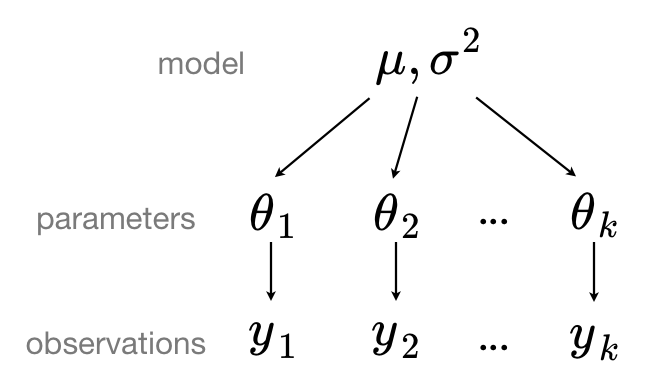
\includegraphics{images/hierarchical.png}
\caption{image}
\end{figure}

Which shows model parameters come from a population distributionm and
each group parameter describes the observations in that group. MCMC
methods allow us to find those parameters by sampling from the posterior
based on the freedom we give to the model. In different situations we
might wish to create difference models with varying levels of
independence. For example, if all flights are limited to the same speed,
then than the relationship between the arrival and departure delay would
have to be fixed for all airlines and any variation in arrival delay
would be due to different intercepts between the airlines.

Markov Chain Monte Carlo methods allow us to approximate the parameters
for our model and are extremely useful when dealing with continuous
variables. In this case, finding the posteriors by hand is impossible
and so we need to use sampling methods for approximate. MCMC can be used
for many different types of Bayesian Inference and we demonstrated how
useful it is for creating hierarchical regression models.


    % Add a bibliography block to the postdoc
    
    
    
    \end{document}
